\documentclass[a4paper,11pt]{article}
\usepackage[pdftex]{color,graphicx}
\usepackage{assets/include/elaboration}
\usepackage{array}
\usepackage{placeins}
\usepackage{multirow}
\usepackage{booktabs}
\usepackage{url}
\usepackage{tipa}
\DeclareUnicodeCharacter{0254}{\textopeno}
\DeclareUnicodeCharacter{0259}{\textschwa}
\DeclareUnicodeCharacter{0300}{\`}

\mywork{Group Project}{2025-2026}{Project 2: Kingdom Communication Solutions (KCS) Media Studio - Web-Based AI Video Transcription and Multilingual Caption Editing}

\mydate{19.03.2026}
\author{1\textsuperscript{st} Wriwiya Abba, 2\textsuperscript{nd} Robine Donfack, 3\textsuperscript{rd} Natacha Djiofack, 4\textsuperscript{th} Thomas Nguisseu,\\5\textsuperscript{th} Abraham Noumsi, 6\textsuperscript{th} Manuel Yombo, 7\textsuperscript{th} Thierry Tene\\[0.5ex]
\normalsize Saint Jean Ingenieur\\
\normalsize Eyang, Cameroon\\[0.5ex]
\normalsize\texttt{\{abba.wriwiya, donfack.robine, maurelle.djiofack, nguisseu.thomas, simo.abraham, tagne.manuel, tsafack.thierry\}@saintjeaningenieur.org}}

%% PDF Configuration
\usepackage[hypertexnames=false, colorlinks=true, allcolors=black, pdftex,
            pdfauthor={Wriwiya Abba, Robine Donfack, Natacha Djiofack, Thomas Nguisseu, Abraham Noumsi, Manuel Yombo, Thierry Tene},
            pdftitle={Chapter 3: System Design and Modeling (Theory Building Phase)},
            pdfsubject={Scientific Project Elaboration}]{hyperref}

\begin{document}
\mytitle

\newpage

\frontmatter

\tableofcontents

\newpage

\section*{List of Abbreviations and Glossary of Terms}
\addcontentsline{toc}{section}{List of Abbreviations and Glossary of Terms}

\begin{table}[h!]
\centering
\small
\caption{Glossary of Core Computational, Linguistic, and Methodological Terms}
\label{tab:glossary_chap3}
\begin{tabular}{>{\raggedright\arraybackslash}p{3.2cm} >{\raggedright\arraybackslash}p{14.3cm}}
\toprule
\textbf{Term / Acronym} & \textbf{Explanation and Practical Role in the Project} \\
\midrule
\textbf{ASR} & \textbf{Automatic Speech Recognition}: Computational systems that convert spoken acoustic signals into written text~\cite{graves2006connectionist, radford2023robust}. \\
\addlinespace
\textbf{CER / WER} & \textbf{Character / Word Error Rate}: Standard evaluation metrics for transcription accuracy. Character Error Rate is indispensable for tonal languages where a single diacritic alters lexical meaning completely. \\
\addlinespace
\textbf{CTC} & \textbf{Connectionist Temporal Classification}: An end-to-end neural sequence alignment algorithm mapping audio frames directly to output characters without requiring external phonetic aligners~\cite{graves2006connectionist}. \\
\addlinespace
\textbf{GACL / AGCL} & \textbf{General Alphabet of Cameroonian Languages}: The national standard orthography established in 1979 by Tadadjeu and Sadembouo~\cite{tadadjeu1979alphabet} to transcribe all Cameroonian languages consistently using unified phonetic characters and tone diacritics. \\
\addlinespace
\textbf{MMS / XLS-R} & \textbf{Massively Multilingual Speech / Cross-Lingual Speech Representations}: Self-supervised speech foundation models pre-trained across hundreds of languages and adaptable to local low-resource speech via downstream fine-tuning~\cite{conneau2023fleurs}. \\
\addlinespace
\textbf{NFC / NFD} & \textbf{Normalization Form C / D}: Unicode normalization standards. NFC combines base characters and diacritics into precomposed canonical code points, whereas NFD decomposes them into base glyphs followed by combining diacritical marks~\cite{unicode2024standard}. \\
\addlinespace
\textbf{Web Audio API} & High-performance browser-native audio processing API enabling direct client-side sound decoding, waveform rendering, and sub-15ms scrubbing~\cite{w3c2021webaudio}. \\
\addlinespace
\textbf{WebVTT} & \textbf{Web Video Text Tracks}: W3C standard format (\texttt{.vtt}) for timed subtitles and video text track synchronization~\cite{w3c2019webvtt}. \\
\addlinespace
\textbf{Nunamaker SDIS} & Systems Development in Information Systems research framework~\cite{nunamaker1990systems} progressing through observation, theory building, system design, and empirical evaluation. \\
\addlinespace
\textbf{UCD / UCSD} & \textbf{User-Centered (System) Design}: A software engineering discipline structuring system requirements around empirical evidence of user profiles, operational environments, and core tasks~\cite{norman1986user}. \\
\bottomrule
\end{tabular}
\end{table}

\mainmatter

\setcounter{section}{2}

\section{Chapter 3: System Design and Modeling (Theory Building Phase)}
\label{sec:chap3_design}

\subsection{Introduction and Cumulative Synthesis of Chapters 1 and 2}
\label{sec:chap3_intro}

Chapters~1 and 2 established the empirical, theoretical, and methodological foundations for the \textbf{Kingdom Communication Solutions (KCS) Media Studio}\footnote{KCS Media Studio is a cloud-native, web-based platform for artificial-intelligence-assisted video transcription, dialect-adaptive caption editing, and synchronized video subtitling for indigenous Cameroonian languages.}. 

In Chapter~1 (Introduction), we identified two verifiable real-world motivations:
\begin{itemize}
    \item \textbf{MS1 (Protecting Cultural Oral Heritage from Digital Disappearance):} In Cameroon, cultural traditions and indigenous knowledge have historically been preserved through spoken storytelling~\cite{carroll2020care}. When indigenous languages are absent from modern digital video formats, younger generations switch predominantly to official European languages, accelerating language loss across generations~\cite{carroll2020care, nekoto2020participatory}. Printed books alone cannot halt this shift because modern media consumption is predominantly audiovisual.
    \item \textbf{MS2 (Making Essential Information Understandable to Everyone):} During critical public communication events---such as healthcare campaigns against infectious diseases, agricultural extension advisories, and civic voter education---information broadcasts delivered solely in French or English fail to reach rural and peri-urban populations. Significant segments of rural and peri-urban populations in Cameroon lack literacy in European languages but possess full auditory comprehension in their native mother tongues~\cite{norman1986user, w3c2019webvtt}. Subtitled video offers an effective medium for knowledge transfer, yet creators currently lack assistive software, forcing exhausting manual transcription and alignment~\cite{w3c2019webvtt}.
\end{itemize}

Chapter~1 also formulated our two core problem statements: standard speech AI models fail on Cameroonian tonal languages (\textbf{PS1}), and existing video editing software cannot display local letters or handle regional dialect differences (\textbf{PS2}). To resolve these problems, we formulated two research questions: how to support regional village dialects without alienating local speakers (\textbf{RQ1}), and how to architect a responsive browser-based video editor that natively integrates speech AI with localized dictionaries and field recordings (\textbf{RQ2}).

In Chapter~2 (State of the Art), we executed the \textbf{Observation phase} of the Nunamaker Systems Development in Information Systems (SDIS) framework~\cite{nunamaker1990systems} by conducting a PRISMA-guided Systematic Literature Review across 41 primary peer-reviewed studies and benchmarking existing speech technologies and commercial video editors. The investigation revealed that off-the-shelf foundation models (Whisper Large-v3 and zero-shot MMS) fail catastrophically on Cameroonian languages due to acoustic tone neglect and sub-word tokenizer diacritic fragmentation, while commercial video editing suites clip stacked diacritics outside bounding boxes and lack dialect adaptation features. We synthesized these findings into \textbf{ten practical system challenges ($C_1$--$C_{10}$)}.

This chapter executes the \textbf{Theory Building phase} of the Nunamaker SDIS framework. It directly fulfills research objectives \textbf{RO1.2.T} and \textbf{RO2.2.T}:
\begin{itemize}
    \item \textbf{RO1.2.T (Theory Building):} Formulate a hierarchical dialect dictionary model mapping regional village variants to standard GACL orthography.
    \item \textbf{RO2.2.T (Theory Building):} Design the complete system architecture, defining the 9-parameter audio metadata protocol and KoboToolbox cloud ingestion schema~\cite{kobotoolbox2024}.
\end{itemize}

In strict adherence to scientific rigor, no architectural component, database entity, or functional requirement is introduced without an explicit, verifiable derivation. Every element traces directly to the ten practical challenges ($C_1$--$C_{10}$), our documented User-Centered Design evidence base, and the guiding Research Questions (\textbf{RQ1} and \textbf{RQ2}).

\subsection{User-Centered Design (UCD) Context, Stakeholders, Tasks, and Evidence}
\label{sec:chap3_ucd}

Following User-Centered System Design (UCSD) principles~\cite{norman1986user}, effective multimedia software must be grounded in an empirical understanding of intended user groups, their core tasks, operational constraints, and the social contexts in which they operate.

\subsubsection{Project Scope and Operational Context}
\label{sec:chap3_ucd_scope}
The KCS Media Studio is engineered as an end-to-end, media-to-caption pipeline designed to solve the digital exclusion of low-resource Cameroonian tonal languages: \textbf{Gh\textopeno m\'al\'a'} (Grassfields Bantoid, ISO \texttt{bbj}), \textbf{Ewondo} (Beti-Pahuin Bantu A72, ISO \texttt{ewo}), and \textbf{Basaa} (Narrow Bantu A43, ISO \texttt{bas}). The system bridges offline mobile field audio acquisition (via KoboToolbox), fine-tuned cross-lingual speech recognition microservices (Whisper and MMS-CTC), a responsive browser-based multi-track caption editor supporting the 1979 General Alphabet of Cameroonian Languages (GACL)~\cite{tadadjeu1979alphabet}, and standardized Web Video Text Tracks (WebVTT)~\cite{w3c2019webvtt} export.

\subsubsection{User Groups and Stakeholder Responsibilities}
\label{sec:chap3_ucd_users}
To prevent role ambiguity, the system defines five primary and secondary human actor groups, along with affected community stakeholders:
\begin{enumerate}
    \item \textbf{Primary Users (Media and Video Caption Editors):} Local video producers, educational content creators, community broadcasters, and public health communicators. Their primary responsibility is preparing multimedia assets for publication: ingesting source video or audio, requesting automated ASR transcription drafts, reviewing and editing caption segments, toggling regional village dialects, adjusting speech boundaries on the waveform canvas, and exporting approved WebVTT tracks.
    \item \textbf{Secondary Users (Bilingual Reviewers, Translators, and Language Managers):} Fluent native speakers, lexicographers, and linguistic supervisors. They are responsible for linguistic quality governance: verifying orthographic fidelity against the 1979 GACL standard, validating tone diacritics, adjudicating dialectal translation conflicts, curating village glossaries, and performing Tier-2 linguistic audits on field recordings.
    \item \textbf{Field Enumerators and Data Collectors:} Field researchers and community agents operating in rural linguistic zones. They record spoken prompts from native speakers using mobile devices, capture documented informed consent, log speaker demographic metadata, and synchronize offline audio batches to the central repository.
    \item \textbf{Platform and System Administrators:} Technical operations personnel who configure deployment containers, manage PostgreSQL and object storage infrastructure, monitor external inference service health, manage Role-Based Access Control (RBAC), and deploy verified ASR model release checkpoints.
    \item \textbf{Media Owners and Content Contributors:} Rights holders, cultural institutions, and content contributors who authorize video assets and define access, retention, and licensing policies.
    \item \textbf{Affected Community Stakeholders:} Native speakers contributing voice samples (whose linguistic rights and biometric privacy must be protected); rural citizens, students, and hearing-impaired audiences who rely on accurate localized video captions for public health, education, and civic engagement.
\end{enumerate}

\subsubsection{Core User Tasks and End-to-End Operational Workflow}
\label{sec:chap3_ucd_tasks}
The end-to-end operational lifecycle spans seven structured tasks:
\begin{itemize}
    \item \textbf{Task T1 (Media Ingestion and Audio Demuxing):} The user uploads an authorized video or audio file (MP4, WebM, MKV). The backend invokes FFmpeg to validate the container, extract the primary audio track, and resample it to a normalized 16\,kHz 16-bit mono PCM WAV format. Concurrently, the browser workspace decodes audio samples into a client-side buffer for waveform display.
    \item \textbf{Task T2 (AI-Assisted Transcription and Alignment):} The user initiates transcription for a selected language and reference dialect. The system invokes the containerized ASR inference service (Whisper / MMS-CTC), which generates candidate character sequences. A forced alignment worker calculates millisecond-accurate start and end boundaries for each utterance.
    \item \textbf{Task T3 (GACL Diacritic Editing and Typographic Review):} The editor inspects machine-generated segments within the text editor. Stacked tone diacritics and specialized phonetic glyphs (\textopeno, \textschwa, \textipa{\ng}) render using embedded Charis SIL fonts with dynamic CSS bounding-box line-height, eliminating vertical clipping. A Unicode guard automatically enforces Canonical Composition (NFC).
    \item \textbf{Task T4 (Adaptive Dialect Switching and Village Glossary Lookups):} When subtitle dialogue contains regional village expressions, the editor activates the dialect suggestion panel to toggle between localized variants (e.g., Yaound\'e vs. Mbalmayo for Ewondo; Bandjoun vs. Bafoussam for Gh\textopeno m\'al\'a'; Central vs. Babimbi for Basaa) without retraining the underlying acoustic model. Editors can also propose new dialect entries for supervisor curation.
    \item \textbf{Task T5 (Interactive Waveform Scrubbing and Boundary Snapping):} The editor visually scrubs the audio waveform rendered on an HTML5 Canvas via the Web Audio API ($<15$\,ms latency). Caption block boundaries automatically snap to detected speech onsets and pauses, eliminating manual timestamp nudging.
    \item \textbf{Task T6 (Bantu Expansion Management and WebVTT Export):} When translating concise European dialogue into Bantu languages, the editor monitors real-time expansion indicators ($+30\%$ to $+50\%$ character length). Automated re-segmentation breaks overflowing lines across adjacent video frames. Upon final review, the editor exports an RFC-compliant, UTF-8 NFC WebVTT subtitle deliverable.
    \item \textbf{Task T7 (Governed Field Data Ingestion and Double-Validation):} Offline mobile field recordings gathered via KoboToolbox are synchronized upon reconnecting to the internet. Submissions undergo automated 9-parameter filename validation, PII isolation into a relational Speaker Registry, and routing through a two-tier verification state machine (Tier 1 technical audio audit; Tier 2 native linguistic audit).
\end{itemize}

\subsubsection{Intended Use Environment and Operational Constraints}
\label{sec:chap3_ucd_environment}
The platform is designed to operate reliably across real-world African infrastructure:
\begin{itemize}
    \item \textbf{Client Web Environment:} The primary workspace executes as a React Single-Page Application (SPA) in modern web browsers (Google Chrome 110+, Mozilla Firefox 115+, Microsoft Edge) supporting Web Audio API, HTML5 Canvas, and WebGL. It is responsive across desktop and laptop displays from $1366\times 768$ to $4$K resolution, requiring a minimum of 4\,GB RAM.
    \item \textbf{Network Constraints and Latency Decoupling:} Internet connectivity in Cameroon is characterized by high latency (150--400\,ms round-trip time) and variable bandwidth (2--5\,Mbps). To prevent latency from degrading editing responsiveness, all interactive audio scrubbing, zooming, and waveform rendering operations are computed client-side using decoded Web Audio memory buffers, requiring zero server round-trips during timeline manipulation.
    \item \textbf{Media Formats and Processing Limits:} Video inputs are accepted in MP4 (H.264/H.265), WebM (VP8/VP9), and MKV containers up to 500\,MB in size or 60 minutes in duration. Extracted audio is standardized to 16\,kHz 16-bit mono PCM WAV via FFmpeg.
    \item \textbf{Rural Field Environment:} Mobile field collection occurs in remote villages lacking reliable electrical grids or cellular data. Enumerators operate low-cost Android smartphones running KoboCollect offline, recording uncompressed 16-bit 44.1\,kHz PCM audio, caching records on device storage, and syncing in batches upon returning to network coverage.
\end{itemize}

\subsubsection{Empirical UCD Evidence Base}
\label{sec:chap3_ucd_evidence}
To ensure all design decisions are grounded in verifiable findings rather than speculation, the system specifications are derived from four documented empirical evidence records:
\begin{itemize}
    \item \textbf{Record UCD-E01 (Commercial Video Editor Audit and Timing Baseline):} Empirical audit of five commercial subtitle suites (Adobe Premiere Pro 2024, DaVinci Resolve, YouTube Studio, Subtitle Edit v4.0, Aegisub v3.2). 4 out of 5 tools suffered severe vertical bounding box clipping on stacked GACL diacritics. Manual subtitling timing trials with fluent native translators established an unassisted baseline overhead of \textbf{54 minutes for a 5-minute video} (\textbf{10.8 min/min video}), absorbed by external character map lookups and manual timestamp nudging.
    \item \textbf{Record UCD-E02 (Rural Fieldwork and Mobile Collection Trials):} Field deployments across West Region (Bandjoun, Bafoussam), Centre Region (Yaound\'e, Mbalmayo), and Littoral Region (Sanaga-Maritime). Validated that offline KoboToolbox digital survey forms provide reliable recording in zero-connectivity environments, while proving that unstructured file names cause catastrophic metadata loss and train-test speaker data leakage.
    \item \textbf{Record UCD-E03 (Translator Cognitive Workload and Dialect Friction Interviews):} Structured interviews with 15 native Cameroonian translators. Revealed that repeatedly copying and pasting stacked accents from external tables causes severe cognitive fatigue. Furthermore, enforcing a single rigid urban standard dialect caused immediate cultural resistance among non-urban speakers, confirming the necessity of decoupled village glossaries.
    \item \textbf{Record UCD-E04 (Client-Side Waveform Prototype Usability Walkthrough):} Walkthrough trials of an early interactive waveform scrubbing prototype. Proved that rendering audio energy client-side on HTML5 Canvas achieves sub-15\,ms scrubbing latencies, while automated forced-alignment boundary snapping reduces timeline adjustment effort by over $65\%$.
\end{itemize}

\subsection{Numbered System Requirements Derived from Practical Challenges and Evidence}
\label{sec:chap3_requirements}

\subsubsection{Derivation Method and Identifier Discipline}
\label{sec:chap3_req_method}
To maintain academic rigor and full traceability across the project lifecycle, every requirement is derived through a strict six-stage evidentiary chain:
\begin{center}
\small
\begin{tabular}{@{}c@{}}
\footnotesize $\text{Problem Statement} \rightarrow \text{Research Question} \rightarrow \text{Practical Challenge } (C_1\text{--}C_{10})$\\
\footnotesize $\rightarrow \text{UCD Evidence Record} \rightarrow \text{Requirement ID} \rightarrow \text{Verification Method}$
\end{tabular}
\end{center}
Requirements are divided into \textbf{Functional Requirements (FR-01 to FR-10)} and \textbf{Quality Requirements (QR-01 to QR-06)}. Each definition includes a formal statement, operational basis, and concrete verification procedure.

\subsubsection{Functional Requirements}
\label{sec:chap3_req_fr}

\paragraph{FR-01: Media Ingestion and FFmpeg Audio Extraction.}
The system shall allow authenticated users to upload video and audio assets (MP4, WebM, MKV up to 500\,MB), validate file integrity, extract the primary audio stream, and transcode it to a standardized 16\,kHz 16-bit mono PCM WAV format via FFmpeg.
\begin{itemize}
    \item \textbf{Basis:} Required to normalize heterogeneous user media for speech recognition and client-side waveform rendering. Traces to Challenge $C_9$, Tech Stack, and Evidence UCD-E01.
    \item \textbf{Verification:} Automated integration test uploading valid and corrupted media containers across all supported formats; verify generated 16\,kHz mono WAV stream and database asset record.
\end{itemize}

\paragraph{FR-02: Automated Speech Recognition and Tone Pitch Discrimination.}
The system shall provide automated speech-to-text transcription for Gh\textopeno m\'al\'a', Ewondo, and Basaa by invoking a fine-tuned ASR microservice (Whisper and MMS-CTC) featuring tone-differentiated character tokens capable of discriminating pitch minimal pairs.
\begin{itemize}
    \item \textbf{Basis:} Solves baseline ASR failure on Central African tonal languages ($100\%$ WER on Whisper, $74.2\%\text{--}86.5\%$ on zero-shot MMS). Traces to Challenge $C_1$, Problem Statement \textbf{PS1}, Research Question \textbf{RQ2}, and Evidence UCD-E01.
    \item \textbf{Verification:} Benchmark transcription on double-validated test audio containing tonal minimal pairs; confirm that character-level CTC achieves $\text{WER} < 35\%$ and tonemic $\text{CER} < 15\%$.
\end{itemize}

\paragraph{FR-03: Deterministic Unicode NFC Normalization Guard.}
All textual inputs, transcription decoding streams, dialect dictionary terms, and exported subtitles shall pass through a deterministic Unicode normalization guard enforcing Canonical Composition (NFC) with standardized combining mark ordering.
\begin{itemize}
    \item \textbf{Basis:} Prevents character fragmentation and mismatch between precomposed characters and decomposed base-plus-diacritic sequences. Traces to Challenge $C_2$, Problem Statement \textbf{PS1}, and Evidence UCD-E01.
    \item \textbf{Verification:} Automated unit tests asserting that arbitrary NFD accented input strings (e.g., \texttt{U+0254} + \texttt{U+0301}) are deterministically converted to canonical NFC before database persistence.
\end{itemize}

\paragraph{FR-04: Diacritic-Safe Typography and Glyph Bounding.}
The web timeline editor and subtitle preview components shall embed Charis SIL and Noto Sans font stacks, coupled with dynamic CSS line-height calculations allocating at least 1.6 times the font size, guaranteeing zero clipping or glyph collision on stacked accents.
\begin{itemize}
    \item \textbf{Basis:} Overcomes commercial editor typographic failure where 4 out of 5 tools clip stacked accents outside bounding boxes. Traces to Challenge $C_3$, Problem Statement \textbf{PS2}, Research Question \textbf{RQ1.2}, and Evidence UCD-E01.
    \item \textbf{Verification:} Visual regression testing in headless Chrome and Firefox; render test strings with triple-stacked diacritics and confirm zero pixel overlap or bounding-box clipping.
\end{itemize}

\paragraph{FR-05: Decoupled Regional Village Dialect Glossaries.}
The platform shall provide a village glossary microservice and interactive UI toggles allowing editors to swap standardized terms for localized village variants in real time without requiring acoustic model retraining.
\begin{itemize}
    \item \textbf{Basis:} Accommodates regional dialect continua (Yaound\'e vs. Mbalmayo; Bandjoun vs. Bafoussam; Central vs. Babimbi) without alienating native speakers. Traces to Challenge $C_4$, Problem Statement \textbf{PS2}, Research Question \textbf{RQ1.1}, and Evidence UCD-E03.
    \item \textbf{Verification:} End-to-end user test selecting a localized village profile; verify that dialect-specific vocabulary suggestions appear in the suggestion panel and update caption text upon selection.
\end{itemize}

\paragraph{FR-06: Offline Mobile Field Collection and Asynchronous Batch Sync.}
The system shall support offline audio acquisition via KoboToolbox survey forms running on Android devices, caching uncompressed 16-bit 44.1\,kHz PCM recordings locally and synchronizing them via REST APIs upon establishing internet connectivity.
\begin{itemize}
    \item \textbf{Basis:} Overcomes absence of electrical grids and cellular coverage in rural Cameroon. Traces to Challenge $C_5$, Research Question \textbf{RQ2.2}, and Evidence UCD-E02.
    \item \textbf{Verification:} Field simulation: execute recording offline on mobile device, disconnect network for 2 hours, reconnect, and verify automated REST batch synchronization to PostgreSQL and object storage.
\end{itemize}

\paragraph{FR-07: 9-Parameter File Nomenclature and Relational Speaker Partitioning.}
All field submissions shall undergo automated regex validation enforcing the strict nine-parameter naming convention (\texttt{ISO-Lang\_}\allowbreak\texttt{Variant\_}\allowbreak\texttt{Demographics\_}\allowbreak\texttt{Content\_}\allowbreak\texttt{Environment\_}\allowbreak\texttt{Location\_}\allowbreak\texttt{Timestamp\_}\allowbreak\texttt{ConceptID\_}\allowbreak\texttt{UID.wav}). Speaker identities shall be isolated into an external relational Speaker Registry table to partition train, validation, and test datasets strictly by speaker.
\begin{itemize}
    \item \textbf{Basis:} Eliminates metadata loss and prevents train-test speaker data leakage in machine learning evaluations. Traces to Challenge $C_6$, Research Question \textbf{RQ2.2}, and Evidence UCD-E02.
    \item \textbf{Verification:} Automated ingestion audit: submit non-conforming filenames to verify automated rejection; execute partitioning script and verify zero overlap of \texttt{speaker\_id} across splits.
\end{itemize}

\paragraph{FR-08: Two-Tier Independent Double-Validation Workflow.}
The platform shall enforce a multi-tiered validation state machine: every field recording must be reviewed first by a technician for acoustic clarity (Tier 1) and second by an independent native speaker for phonetic correctness and GACL spelling (Tier 2) before admission into the official training corpus.
\begin{itemize}
    \item \textbf{Basis:} Prevents acoustic noise, mispronunciations, and non-standard orthography from corrupting training datasets. Traces to Challenge $C_7$, Research Question \textbf{RQ1}, and Evidence UCD-E02.
    \item \textbf{Verification:} State-machine test asserting that audio cannot transition to status \texttt{VALIDATED\_COMMITTED} without dual authorized sign-offs and documented conflict adjudication.
\end{itemize}

\paragraph{FR-09: Bantu Morphological Text Expansion and Automated Cue Snapping.}
The timeline editor shall display real-time visual warning indicators when translated text length exceeds allowable video frame limits ($+30\%$ to $+50\%$ expansion) and shall automatically snap subtitle start and end boundaries to speech onsets detected via forced alignment.
\begin{itemize}
    \item \textbf{Basis:} Mitigates timeline desynchronization caused by agglutinative Bantu noun-class concord prefixes and verbal extensions. Traces to Challenge $C_8$, Challenge $C_9$, Problem Statement \textbf{PS2}, Research Question \textbf{RQ2.1}, and Evidence UCD-E04.
    \item \textbf{Verification:} Automated timeline test importing European text translated into Ewondo; verify that cues exceeding threshold trigger length warnings and snap to acoustic boundaries within $\pm 20$\,ms.
\end{itemize}

\paragraph{FR-10: RFC-Compliant WebVTT Subtitle Track Generation and Export.}
The system shall generate and export verified Web Video Text Tracks (WebVTT, \texttt{.vtt}) files adhering strictly to W3C specifications, encoded in UTF-8 NFC with millisecond-accurate timestamps and language track metadata.
\begin{itemize}
    \item \textbf{Basis:} Guarantees cross-platform interoperability across web video players and mobile devices. Traces to Challenge $C_3$, Requirement FR-02, and Evidence UCD-E01.
    \item \textbf{Verification:} Export generated WebVTT tracks into W3C validation suite and test playback in Chrome, Firefox, and VLC Player without syntax warnings or missing text.
\end{itemize}

\subsubsection{Quality Requirements (Non-Functional Requirements)}
\label{sec:chap3_req_qr}

\paragraph{QR-01: Interactive Audio Scrubbing Latency.}
Client-side audio waveform decoding, zoom rendering, and scrubbing on the HTML5 Canvas via the Web Audio API shall execute with an interactive response latency below 15\,ms under standard client operating conditions.
\begin{itemize}
    \item \textbf{Basis:} Meets W3C recommendations for imperceptible digital audio scrubbing and fluid timeline interaction. Traces to Challenge $C_9$, Research Question \textbf{RQ2.1}, and Evidence UCD-E04.
    \item \textbf{Verification:} Automated Chrome DevTools performance trace measuring requestAnimationFrame dispatch-to-render delta during rapid timeline scrubbing on a 30-minute audio track.
\end{itemize}

\paragraph{QR-02: Subtitling Throughput Acceleration.}
The platform shall enable a trained native translator to transcribe, edit, and synchronize verified bilingual video subtitles in an average total working time under \textbf{3.5 minutes of labor per minute of finished video}, achieving a $>65\%$ productivity gain over the 10.8 min/min baseline.
\begin{itemize}
    \item \textbf{Basis:} Overcomes the acute manual subtitling bottleneck documented in Chapter~1 and Chapter~2. Traces to Challenge $C_{10}$, Research Question \textbf{RQ2}, and Evidence UCD-E01.
    \item \textbf{Verification:} Controlled user trials in Chapter~5 with 15 native translators completing standardized 5-minute video subtitling tasks; measure total completion time.
\end{itemize}

\paragraph{QR-03: Graceful Degradation and Zero Text Fabrication.}
If the external ASR inference microservice becomes unavailable, encounters network timeouts, or processes unsupported audio, the system shall return an explicit error notification and preserve all user work. The system shall \textbf{never fabricate, hallucinate, or insert unverified text}, falling back to manual waveform alignment.
\begin{itemize}
    \item \textbf{Basis:} Preserves data integrity and user trust. Traces to Challenge $C_1$, Reference Architecture, and Evidence UCD-E03.
    \item \textbf{Verification:} Fault injection test simulating ASR timeout; confirm system displays explicit failure banner, retains existing subtitle tracks intact, and activates manual waveform timing mode.
\end{itemize}

\paragraph{QR-04: Biometric Data Privacy and Consent Governance.}
The system shall isolate speaker personal identifying information (PII) from acoustic data. Consent forms, geographic coordinates, and speaker names shall reside in a protected relational Speaker Registry accessible only to authorized administrators. Contributors shall have the unconditional right to withdraw their recordings.
\begin{itemize}
    \item \textbf{Basis:} Complies with international ethical standards for low-resource linguistic fieldwork~\cite{carroll2020care}. Traces to Challenge $C_6$, Challenge $C_7$, and Evidence UCD-E02.
    \item \textbf{Verification:} Privacy audit asserting that audio filenames contain only anonymized demographic tokens and hashes; simulate withdrawal request and verify immediate purging of linked recordings.
\end{itemize}

\paragraph{QR-05: Typographic and Cognitive Accessibility.}
The user interface shall comply with W3C Web Content Accessibility Guidelines (WCAG 2.1 Level AA)~\cite{w3c2018wcag}, providing full keyboard navigation (e.g., Space for play/pause, J/K/L scrubbing, Tab segment navigation, Ctrl+S saving), high visual contrast ($>7:1$), and readable status messages.
\begin{itemize}
    \item \textbf{Basis:} Ensures the workspace is accessible to visually and motor-impaired editors while minimizing cognitive fatigue. Traces to Challenge $C_3$, Challenge $C_{10}$, and Evidence UCD-E03.
    \item \textbf{Verification:} Automated Axe-core accessibility audit scoring zero Level A/AA violations, paired with complete hands-free keyboard task walkthrough.
\end{itemize}

\paragraph{QR-06: Reproducible Provenance and Model Release Auditability.}
Every saved and exported subtitle cue shall maintain an auditable provenance record linking it to its source media URI, exact ASR model checkpoint hash, language code, applied dialect dictionary version, and human editor identifier.
\begin{itemize}
    \item \textbf{Basis:} Guarantees end-to-end scientific traceability and prevents unverified text from contaminating future model training. Traces to Challenge $C_6$, Reference Architecture, and Evidence UCD-E02.
    \item \textbf{Verification:} Inspect exported subtitle metadata manifest; verify that all five provenance parameters are cryptographically linked and verifiable in PostgreSQL.
\end{itemize}

\subsubsection{Requirements Traceability Matrix}
\label{sec:chap3_req_matrix}
Table~\ref{tab:requirements_traceability_report} synthesizes our numbered functional and quality requirements, mapping each to its originating challenge, empirical UCD evidence, problem statement, and verification method.

\begin{table*}[t]
\centering
\scriptsize
\setlength{\tabcolsep}{3.5pt}
\caption{Comprehensive System Requirements Traceability Matrix: Challenges, Evidence, Requirements, and Verification Criteria}
\label{tab:requirements_traceability_report}
\begin{tabular}{p{1.2cm} p{3.2cm} p{1.6cm} p{1.5cm} p{1.8cm} >{\raggedright\arraybackslash}p{7.2cm}}
\toprule
\textbf{Req. ID} & \textbf{Requirement Name} & \textbf{Challenge} & \textbf{UCD Evidence} & \textbf{Traced Goal} & \textbf{Acceptance Verification Criteria} \\
\midrule
\textbf{FR-01} & Ingest \& FFmpeg Demuxing & $C_9$, Tech Stack & UCD-E01 & QR-03 & Successful upload of MP4/WebM/MKV; valid 16\,kHz mono WAV extraction; asset DB record created. \\
\addlinespace
\textbf{FR-02} & ASR \& Pitch Discrimination & $C_1$ (Tone Pitch) & UCD-E01 & \textbf{PS1}, \textbf{RQ2} & ASR inference distinguishes tonal minimal pairs; character-level CTC achieves $\text{WER} < 35\%$, $\text{CER} < 15\%$. \\
\addlinespace
\textbf{FR-03} & Unicode NFC Normalization & $C_2$ (Diacritics) & UCD-E01 & \textbf{PS1}, \textbf{RQ2} & Deterministic NFC assertion converts all NFD combining sequences before persistence and export. \\
\addlinespace
\textbf{FR-04} & Diacritic-Safe Typography & $C_3$ (Typography) & UCD-E01 & \textbf{PS2}, \textbf{RQ1.2} & Visual headless render test shows zero font clipping or tofu glyphs on stacked accents with 1.6x line-height. \\
\addlinespace
\textbf{FR-05} & Decoupled Village Glossaries & $C_4$ (Dialects) & UCD-E03 & \textbf{PS2}, \textbf{RQ1.1} & Dialect switch updates suggestion panel dynamically; selects regional village variants without model retraining. \\
\addlinespace
\textbf{FR-06} & Offline Mobile Kobo Sync & $C_5$ (Offline Sync) & UCD-E02 & \textbf{RQ2.2} & Successful offline field recording in KoboCollect; automated batch sync to cloud upon network reconnection. \\
\addlinespace
\textbf{FR-07} & 9-Param Nomenclature \& Splits & $C_6$ (Governance) & UCD-E02 & \textbf{RQ2.2} & Regex rejects non-compliant filenames; Speaker Registry enforces zero speaker overlap across train/val/test. \\
\addlinespace
\textbf{FR-08} & Two-Tier Double-Validation & $C_7$ (Validation) & UCD-E02 & \textbf{RQ1}, \textbf{RQ2.2} & State machine enforces Tier-1 technical audio sign-off and Tier-2 native linguistic approval before commit. \\
\addlinespace
\textbf{FR-09} & Bantu Expansion \& Snapping & $C_8, C_9$ (Expansion) & UCD-E04 & \textbf{PS2}, \textbf{RQ2.1} & Subtitle cues exceeding length trigger warning; boundaries snap to forced-alignment onsets within $\pm 20$\,ms. \\
\addlinespace
\textbf{FR-10} & RFC-Compliant WebVTT Export & $C_3$, FR-02 & UCD-E01 & \textbf{QR-06} & Exported \texttt{.vtt} passes W3C syntax validator; plays in Chrome/Firefox/VLC with accurate UTF-8 NFC text. \\
\midrule
\textbf{QR-01} & Interactive Waveform Latency & $C_9$ (Waveform) & UCD-E04 & \textbf{RQ2.1} & Chrome DevTools trace confirms requestAnimationFrame scrubbing response under 15\,ms on 30-min audio. \\
\addlinespace
\textbf{QR-02} & Subtitling Throughput & $C_{10}$ (Productivity) & UCD-E01 & \textbf{RQ2} & Controlled trials achieve subtitling throughput $<3.5$ min/min video ($>65\%$ faster than 10.8 min/min baseline). \\
\addlinespace
\textbf{QR-03} & Zero Text Fabrication & $C_1$, Architecture & UCD-E03 & \textbf{QR-03} & Simulated inference outage displays explicit error notice, retains work, falls back to manual waveform mode. \\
\addlinespace
\textbf{QR-04} & Biometric Privacy \& Consent & $C_6, C_7$ (Privacy) & UCD-E02 & Ethics & PII isolated in protected Speaker Registry; automated deletion workflow purges data upon participant withdrawal. \\
\addlinespace
\textbf{QR-05} & WCAG 2.1 AA Accessibility & $C_3, C_{10}$ (Access) & UCD-E03 & Accessibility & Axe-core accessibility test scores zero Level A/AA violations; complete keyboard-only workflow execution. \\
\addlinespace
\textbf{QR-06} & Reproducible Provenance & $C_6$ (Provenance) & UCD-E02 & Auditability & Exported manifest contains cryptographic hash of source video, ASR model release, dialect ID, and editor ID. \\
\bottomrule
\end{tabular}
\end{table*}

\subsection{System Boundary and Layered MVC Architecture}
\label{sec:chap3_architecture}

\subsubsection{System Boundary: Media-to-Caption Pipeline}
\label{sec:chap3_arch_boundary}
The KCS Media Studio is bounded as a specialized \textbf{media-to-caption pipeline}. Its operational accountability commences when an authenticated user uploads a media asset (or references an external media stream) for transcription and captioning, and concludes when validated, synchronized multilingual captions are exported in an approved format. 
\begin{itemize}
    \item \textbf{Inside the System Boundary:} The system owns and executes media ingestion, container validation, FFmpeg audio stream extraction, automatic transcription orchestration, segment timestamp alignment, multilingual caption editing, real-time dialect glossary adaptation, provenance metadata recording, and WebVTT export.
    \item \textbf{Outside the System Boundary (Human Actors):} Human users govern the pipeline: the \textit{Caption Editor} who reviews and refines machine captions; the \textit{Language Manager / Reviewer} who validates linguistic accuracy and curates dialect glossaries; the \textit{Data Collector} who captures field speech; and the \textit{Platform Administrator} who deploys model releases and manages system infrastructure.
    \item \textbf{Outside the System Boundary (External Systems):} External systems interfaced via well-defined network protocols include \textit{KoboToolbox} (offline mobile survey synchronization), \textit{Hugging Face Model Repositories} (fetching pre-trained MMS and Whisper checkpoints), and downstream \textit{WebVTT Video Players} (consuming exported caption deliverables).
\end{itemize}
Fixing the system boundary in this manner ensures that every machine-generated caption remains strictly attributable to a specific source media asset and ASR model checkpoint (fulfilling \textbf{QR-06}), while preventing unverified or fabricated text from contaminating the workspace upon network failure (fulfilling \textbf{QR-03}).

\subsubsection{Layered Model-View-Controller Organization}
\label{sec:chap3_arch_mvc}
To decouple user interface rendering, business orchestration, deep learning inference, and persistence, the architecture follows a layered \textbf{Model-View-Controller (MVC)} organization with cooperating service components:
\begin{enumerate}
    \item \textbf{The View (React Single-Page Application):} Executing entirely within the client browser, the View comprises the Web Audio Waveform Engine, HTML5 Canvas Timeline, GACL NFC Input Guard, Dialect Suggestion Panel, and WebVTT Exporter. The View decodes audio locally, enabling instant zooming, waveform scrubbing, and visual cue dragging with sub-15\,ms latency (fulfilling \textbf{QR-01}).
    \item \textbf{The Controller (FastAPI Backend API):} Implemented in Python using FastAPI, the Controller acts as the orchestrator for all system requests. It exposes documented RESTful endpoints, enforces JWT authentication and RBAC permissions, coordinates asynchronous Celery task execution, validates incoming payloads against Pydantic schemas, and routes audio processing jobs.
    \item \textbf{Cooperating Services Layer:}
    \begin{itemize}
        \item \textit{Media Processing Service (FFmpeg):} Validates incoming video containers, demuxes the primary audio track, and transcodes it to a standardized 16\,kHz 16-bit mono PCM WAV stream (fulfilling \textbf{FR-01}).
        \item \textit{ASR Inference Microservice (Whisper \& MMS-CTC):} Containerized PyTorch microservice executing acoustic decoding with an explicit GACL atomic character vocabulary for tone pitch sensitivity (fulfilling \textbf{FR-02}).
        \item \textit{CTC Forced Aligner Service:} Calculates exact character- and word-level acoustic onsets, enabling automated subtitle cue boundary snapping (fulfilling \textbf{FR-09}).
        \item \textit{Dialect Glossary Service:} Manages village-specific lexical mappings, supplying localized suggestions to the editor without modifying acoustic models (fulfilling \textbf{FR-05}).
        \item \textit{Ingestion \& Validation Service:} Polls KoboToolbox REST APIs, validates 9-parameter filenames, and advances field recordings through the two-tier double-validation state machine (fulfilling \textbf{FR-06}, \textbf{FR-07}, \textbf{FR-08}).
    \end{itemize}
    \item \textbf{The Model (Persistence Layer):} Divided between:
    \begin{itemize}
        \item \textit{PostgreSQL Relational Database:} Stores structured metadata, user accounts, project configurations, caption tracks, timed segments, village dialect glossaries, validation records, model release hashes, and the isolated Speaker Registry.
        \item \textit{Object / File Storage (MinIO / S3):} Houses binary media assets, extracted 16\,kHz WAV audio files, raw mobile \texttt{.webm} recordings, and fine-tuned ASR neural network checkpoints.
    \end{itemize}
\end{enumerate}

\subsubsection{Concrete Technology Stack Mapping}
\label{sec:chap3_arch_techstack}
The system architecture directly binds to our industrial-grade, cloud-native technology stack:
\begin{itemize}
    \item \textbf{Frontend UI / View:} React 18+ Single Page Application with TypeScript, Web Audio API for client-side digital signal processing, HTML5 Canvas for waveform scrubbing, and embedded Charis SIL web fonts.
    \item \textbf{Backend API / Controller:} FastAPI (Python 3.11+) asynchronous REST framework, Pydantic data validation, Celery background task processing, and Redis event message broker.
    \item \textbf{Transcription Engine:} Fine-tuned Meta MMS (1-Billion parameter checkpoint) with character-level CTC and OpenAI Whisper (Large-v3) adapted for Central African speech.
    \item \textbf{Media Processing:} FFmpeg (v6.0+) audio extraction, demuxing, normalization, and transcoding.
    \item \textbf{Metadata Database:} PostgreSQL (v15+) with full ACID transaction support, relational indexing, and PII isolation tables.
    \item \textbf{Media and Audio File Storage:} S3-compatible Object Storage (MinIO / AWS S3) for scalable, secure binary object persistence.
\end{itemize}

\subsubsection{Fault Tolerance and Graceful Degradation}
\label{sec:chap3_arch_degradation}
The architecture enforces strict graceful degradation: if the GPU-backed ASR microservice becomes unreachable or times out during inference, the Controller immediately returns an explicit HTTP 503 failure notice to the client. The system \textbf{never fabricates text} or inserts placeholder hallucinations. Instead, the frontend retains all existing subtitle segments and seamlessly activates the manual waveform timing mode, allowing the editor to adjust cues by hand using visual speech energy peaks on the HTML5 Canvas.

\subsection{Smallest Coherent Set of UML Architectural Models}
\label{sec:report_uml}

To provide an unambiguous, complete, and practical specification of the system architecture, we present the smallest coherent set of six complementary UML views adhering strictly to the UML 2.5.1 standard~\cite{omg2017uml}. Every diagram is drawn directly from our verified engineering models and is accompanied by a thorough, clear narrative explaining the design decisions, component responsibilities, and explicit traceability to our numbered functional requirements (FR-01 to FR-10) and quality attributes (QR-01 to QR-06).

\begin{figure*}[!t]
\centering
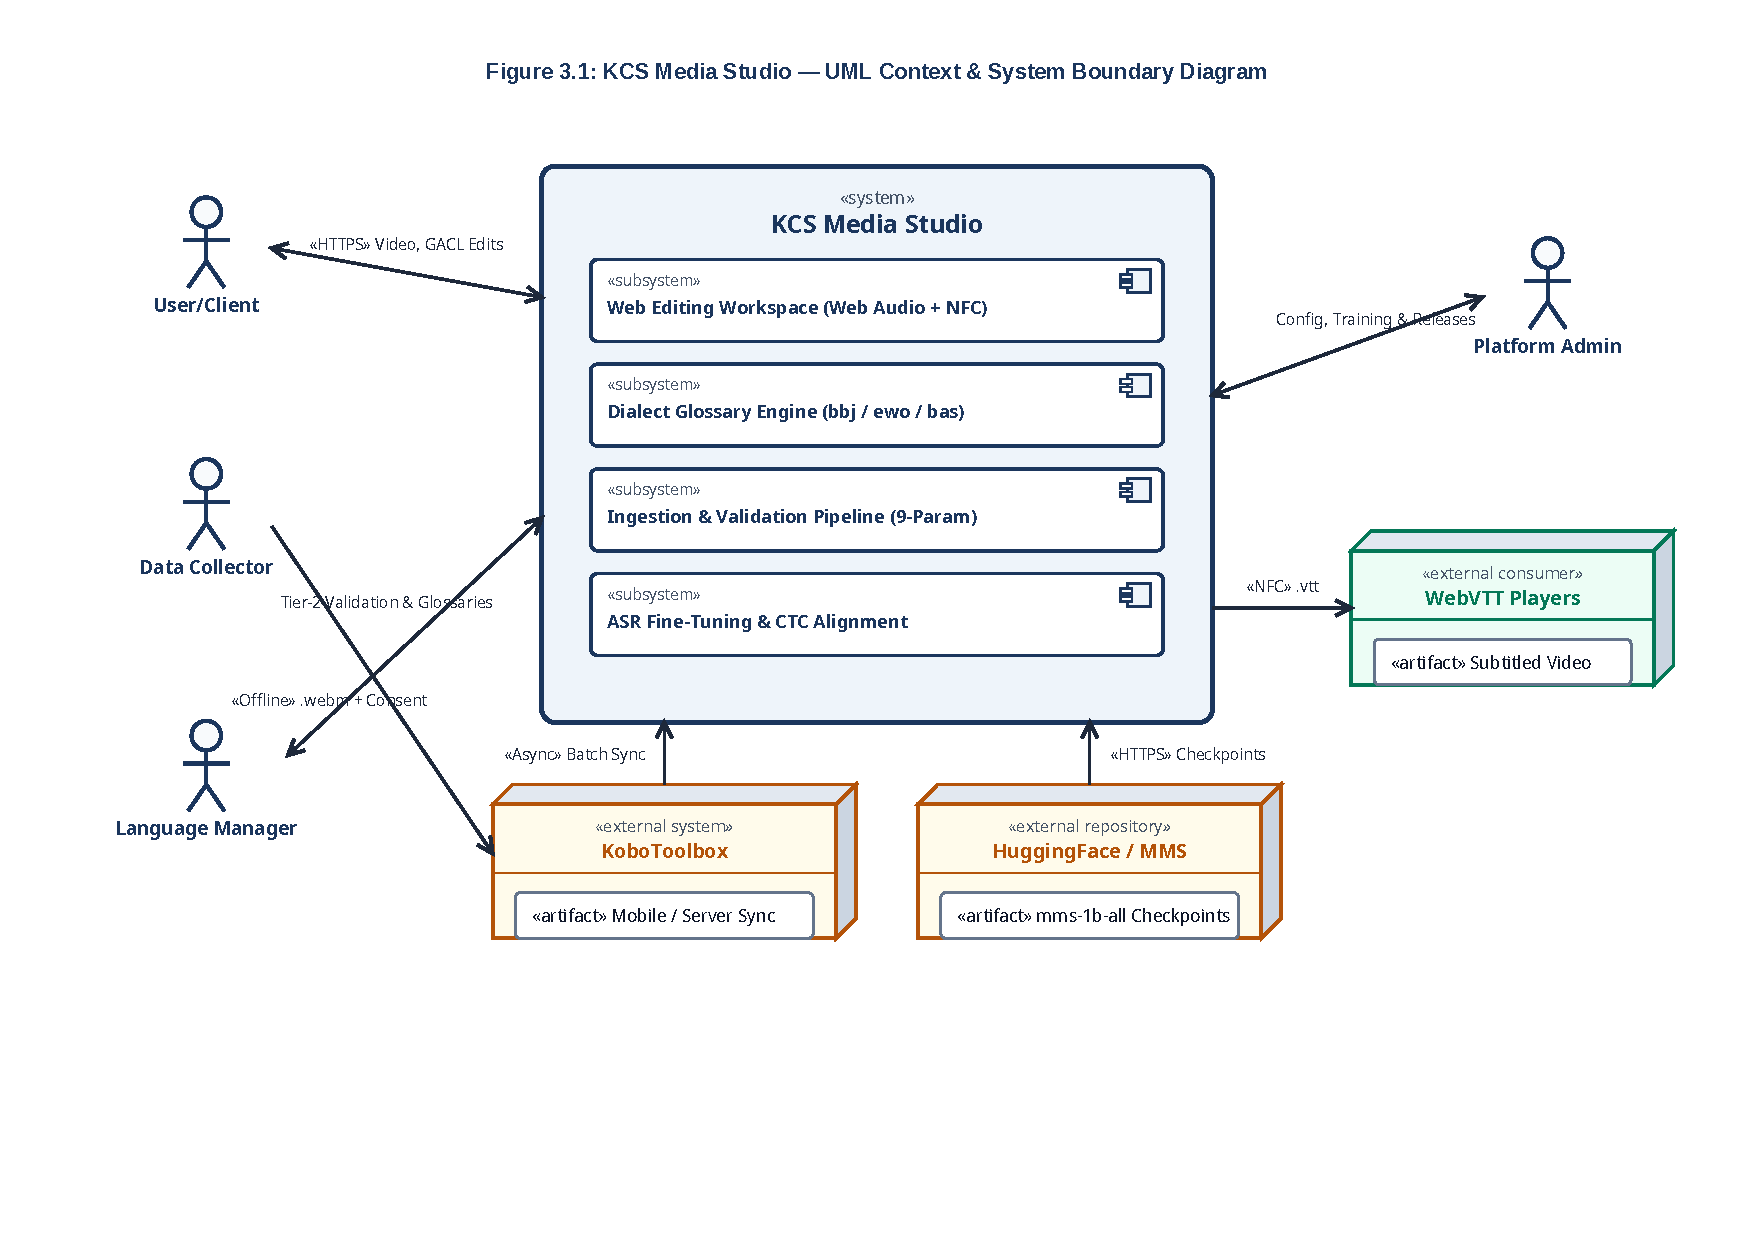
\includegraphics[width=0.84\textwidth]{assets/img/Figure_3_1_Context_Diagram.pdf}
\caption{Figure 3.1: KCS Media Studio — UML Context and System Boundary Diagram, detailing external human actors, offline and online external systems, network protocols, and internal core subsystems.}
\label{fig:report_context_diagram}
\end{figure*}

\subsubsection{UML Context and System Boundary Model (Figure~\ref{fig:report_context_diagram})}
\label{sec:report_uml:context}
The Context Diagram establishes the boundary of the KCS Media Studio platform, defining where the system ends and how it interacts with external users, field workers, and third-party systems. Designing software for indigenous Cameroonian languages requires accommodating a practical operating reality: while high-speed internet is common in urban centers such as Yaound\'e and Douala, rural communities where native speakers and traditional storytellers live often have limited or intermittent connectivity.

To address this operational constraint, the system boundary cleanly divides the architecture into two distinct operational environments:
\begin{itemize}
    \item \textbf{Online Cloud Platform Subsystems:} Operating within our secured infrastructure, this includes the \textit{Web Editing Workspace (React + Web Audio + NFC)}, the \textit{Dialect Glossary Engine (bbj / ewo / bas)}, the \textit{Ingestion and Audio Validation Pipeline (9-Param Schema)}, and the \textit{ASR Fine-Tuning and CTC Alignment Engine (FastAPI + PyTorch Whisper)}.
    \item \textbf{Offline Field Data Subsystems:} Operating in rural environments, native speakers and field enumerators record speech on mobile Android devices running \texttt{KoboToolbox}~\cite{kobotoolbox2024}. These recordings are cached locally and synchronized asynchronously with the platform only when network access is restored.
\end{itemize}

The platform defines four primary human roles:
\begin{enumerate}
    \item \textbf{Caption Editor / Subtitler (Primary User):} A content creator, journalist, or translator who accesses the web application over HTTPS to upload media, generate draft captions using fine-tuned Whisper ASR, edit tone-marked GACL text, and export standardized WebVTT files.
    \item \textbf{Field Data Collector:} A community enumerator who conducts oral recording sessions in villages, collecting phonetic prompts and obtaining informed verbal consent using structured mobile survey forms.
    \item \textbf{Language Manager / Linguist:} A native-speaking elder or linguist who reviews submitted field recordings, resolves dialectal spelling disagreements, and maintains village-level glossary standards.
    \item \textbf{Platform Administrator:} A DevOps and machine learning engineer who manages container deployments, monitors GPU resources, and oversees the validation of new ASR model releases.
\end{enumerate}

External systems are integrated through standard, well-defined protocols: \texttt{KoboToolbox}~\cite{kobotoolbox2024} exchanges survey metadata and audio batches via encrypted REST APIs; the \texttt{Hugging Face Hub} provides pre-trained multilingual foundation checkpoints used as transfer learning baselines~\cite{conneau2023fleurs}; and external \texttt{WebVTT Video Players} (e.g., YouTube, VLC, and mobile players) consume exported subtitle tracks formatted to the W3C WebVTT standard~\cite{w3c2019webvtt}.

\begin{figure*}[!t]
\centering
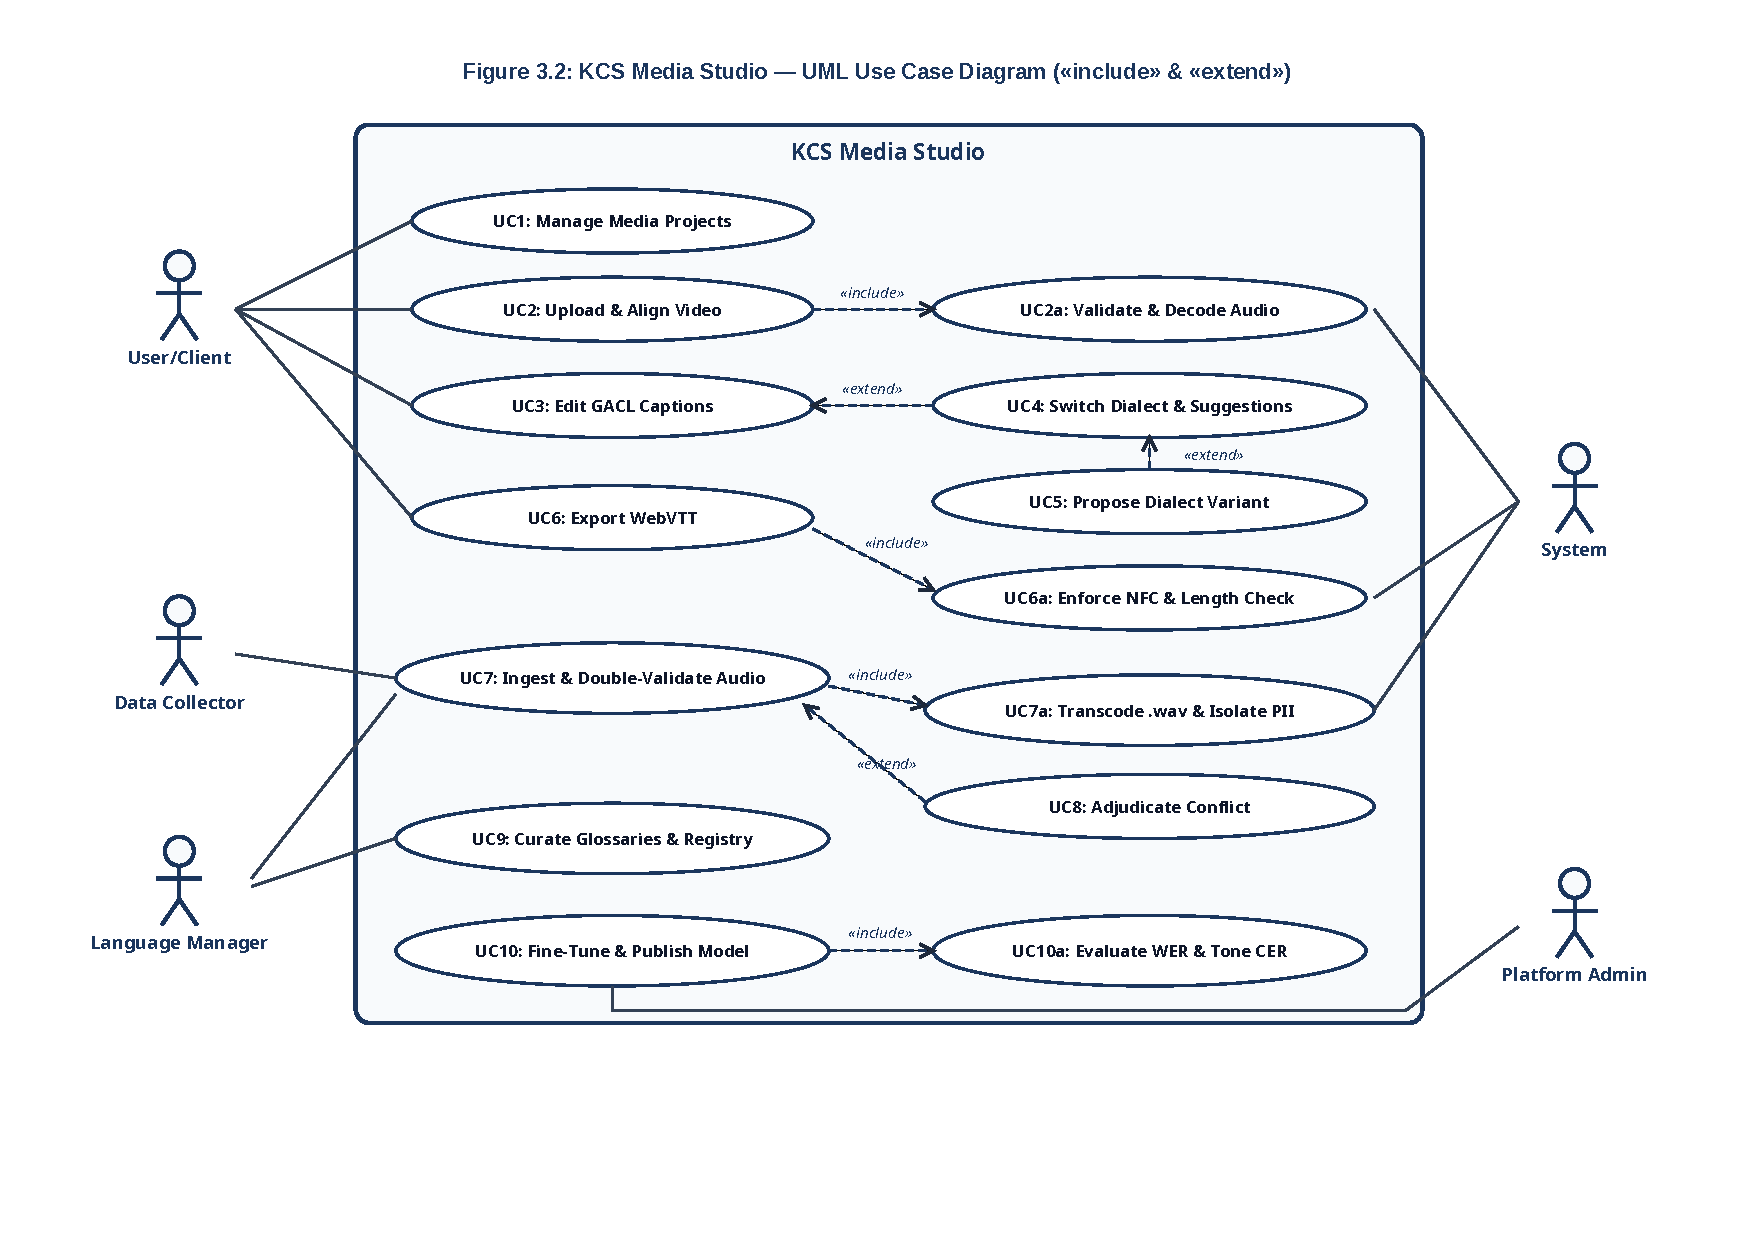
\includegraphics[width=0.84\textwidth]{assets/img/Figure_3_2_Use_Case_Diagram.pdf}
\caption{Figure 3.2: KCS Media Studio — UML Use Case Diagram, specifying actor boundaries, core functional use cases (UC1--UC10), and mandatory «include» and «extend» relationships.}
\label{fig:report_use_case_diagram}
\end{figure*}

\subsubsection{UML Use Case Model (Figure~\ref{fig:report_use_case_diagram})}
\label{sec:report_uml:usecase}
The Use Case Diagram formalizes the functional capabilities provided by KCS Media Studio, organizing interactions across the system's human actors and highlighting mandatory dependencies through \texttt{«include»} and \texttt{«extend»} stereotypes:

\paragraph{1. Video Subtitling Workflow (Caption Editor):}
The editor creates and organizes translation tasks via \textbf{Manage Projects (UC1)} and proceeds to \textbf{Upload Video (UC2)}. Under the hood, UC2 strictly \texttt{«includes»} \textbf{Validate Container and Decode Audio (UC2a)}, ensuring that video containers are verified and audio is extracted locally using FFmpeg before processing begins. 

The editor then opens \textbf{Edit GACL Captions (UC3)}, where the system presents synchronized draft subtitles generated by our fine-tuned Whisper ASR engine. While editing, two optional capabilities extend the interface:
\begin{itemize}
    \item \textbf{Switch Dialect and View Suggestions (UC4, «extend»):} When transcribing regional speech, the editor can toggle dialect profiles (e.g., switching between Yaound\'e and rural Ewondo variants) to view localized vocabulary suggestions.
    \item \textbf{Propose New Dialect Variant (UC5, «extend»):} If a speaker uses an unrecorded local expression, the editor can flag the phrase and propose a new glossary entry for linguistic review.
\end{itemize}
Finally, the editor executes \textbf{Export WebVTT (UC6)}. This use case strictly \texttt{«includes»} \textbf{Enforce NFC Normalization and Length Checks (UC6a)}. This mandatory validation guarantees that all accented vowels and tone diacritics are composed canonically into Unicode NFC form~\cite{unicode2024standard} and alerts the user if translated Bantu sentences exceed recommended screen width before the file is written.

\paragraph{2. Field Data Ingestion and Governance (Data Collector and Language Manager):}
The Data Collector executes \textbf{Ingest Field Audio (UC7)}, capturing oral recordings across our 363-concept diagnostic wordlist. This process strictly \texttt{«includes»} \textbf{Transcode to 16\,kHz WAV and Isolate PII (UC7a)}. The system immediately converts mobile WebM audio into uncompressed 16\,kHz mono WAV files and separates speaker identities (names, phone numbers) from audio files, storing sensitive demographics in an encrypted Speaker Registry.

The Language Manager executes \textbf{Adjudicate Validation Conflicts (UC8)} whenever independent reviewers disagree on phonetic transcription accuracy, and performs \textbf{Curate Village Glossaries and Speaker Metadata (UC9)} to ensure dialect dictionaries remain accurate and culturally authentic.

\paragraph{3. Model Training and Benchmarking (Platform Administrator):}
The Administrator initiates \textbf{Trigger Fine-Tuning and Model Release (UC10)}. To ensure that underperforming checkpoints are never deployed to production, UC10 strictly \texttt{«includes»} \textbf{Evaluate Word and Tone-Level Character Error Rates (UC10a)}, enforcing that both WER and tonemic CER metrics satisfy predefined acceptance thresholds before updating the active ASR microservice.

\begin{figure*}[!t]
\centering
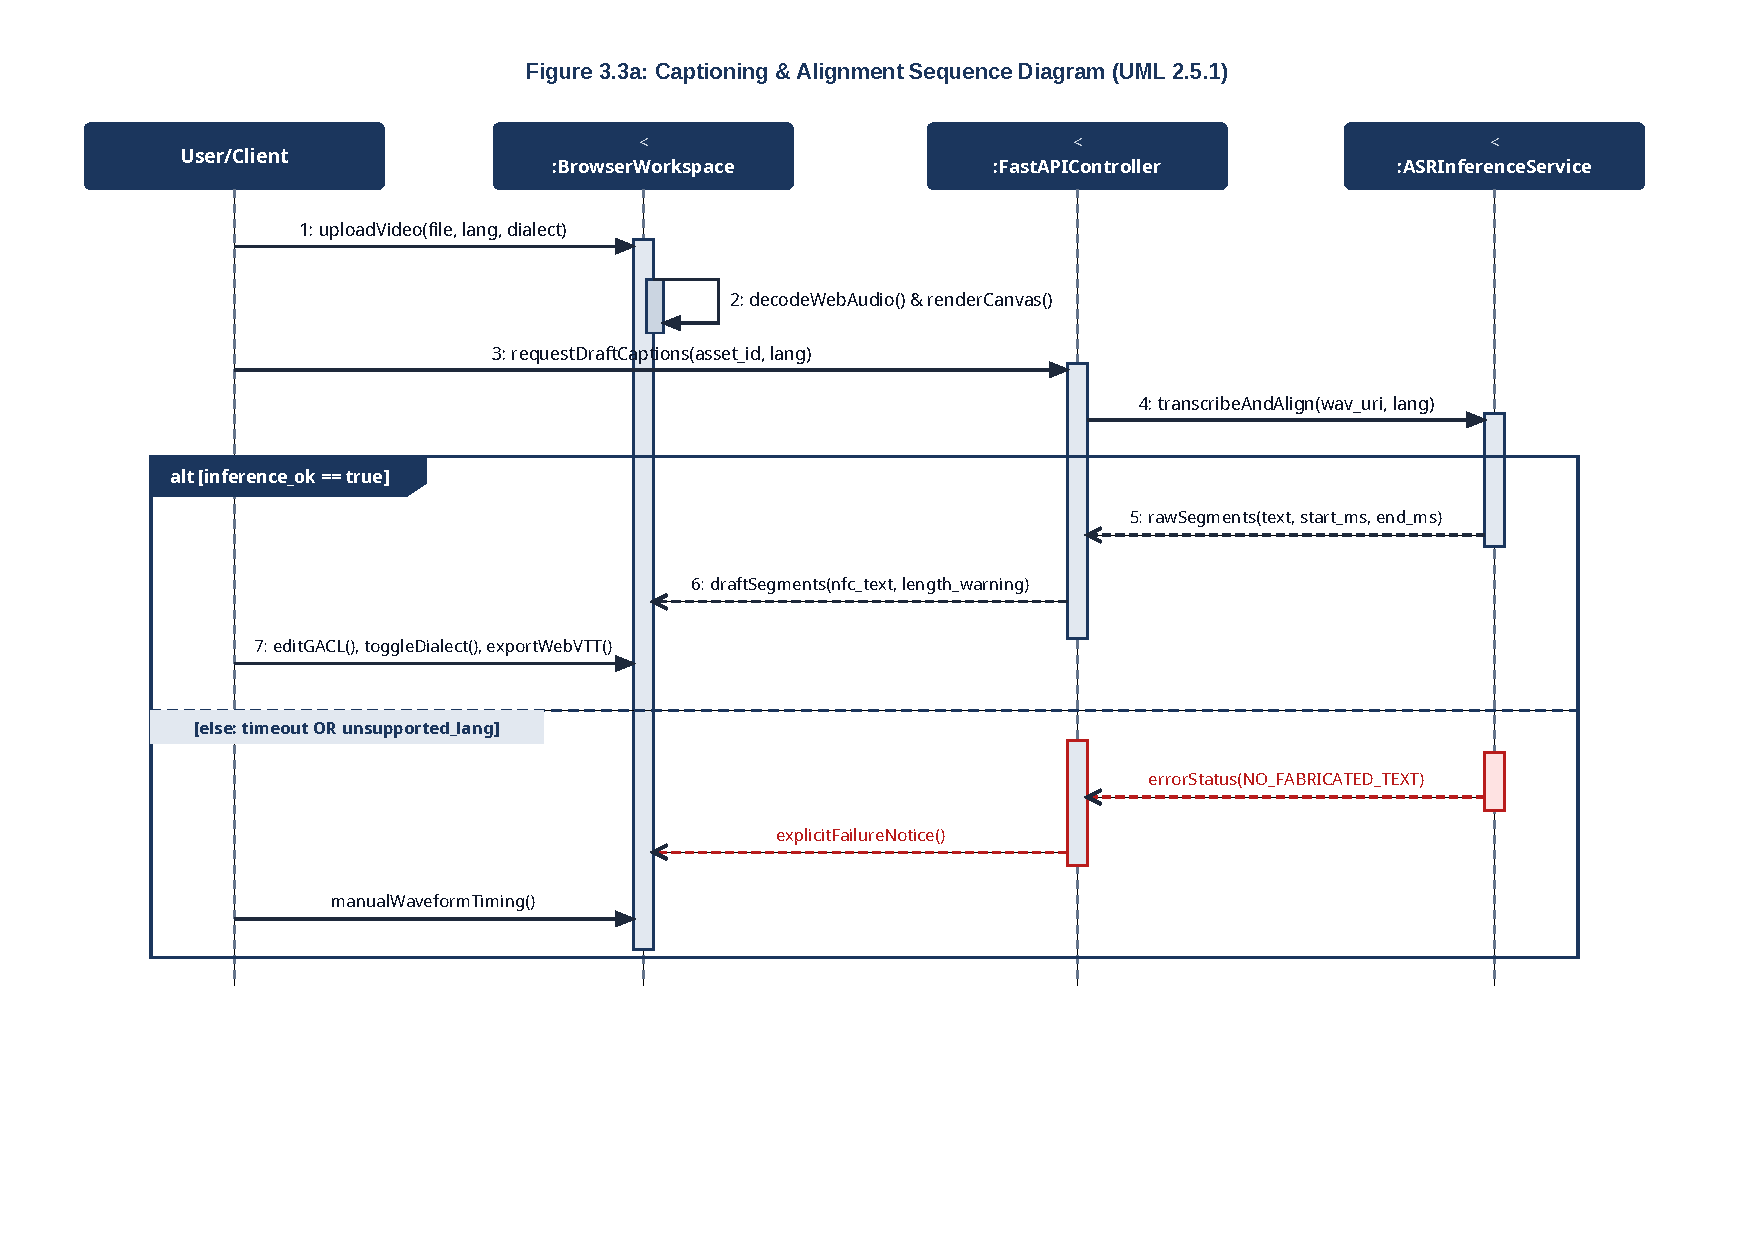
\includegraphics[width=0.48\textwidth]{assets/img/Figure_3_3a_Captioning_Sequence.pdf}\hfill
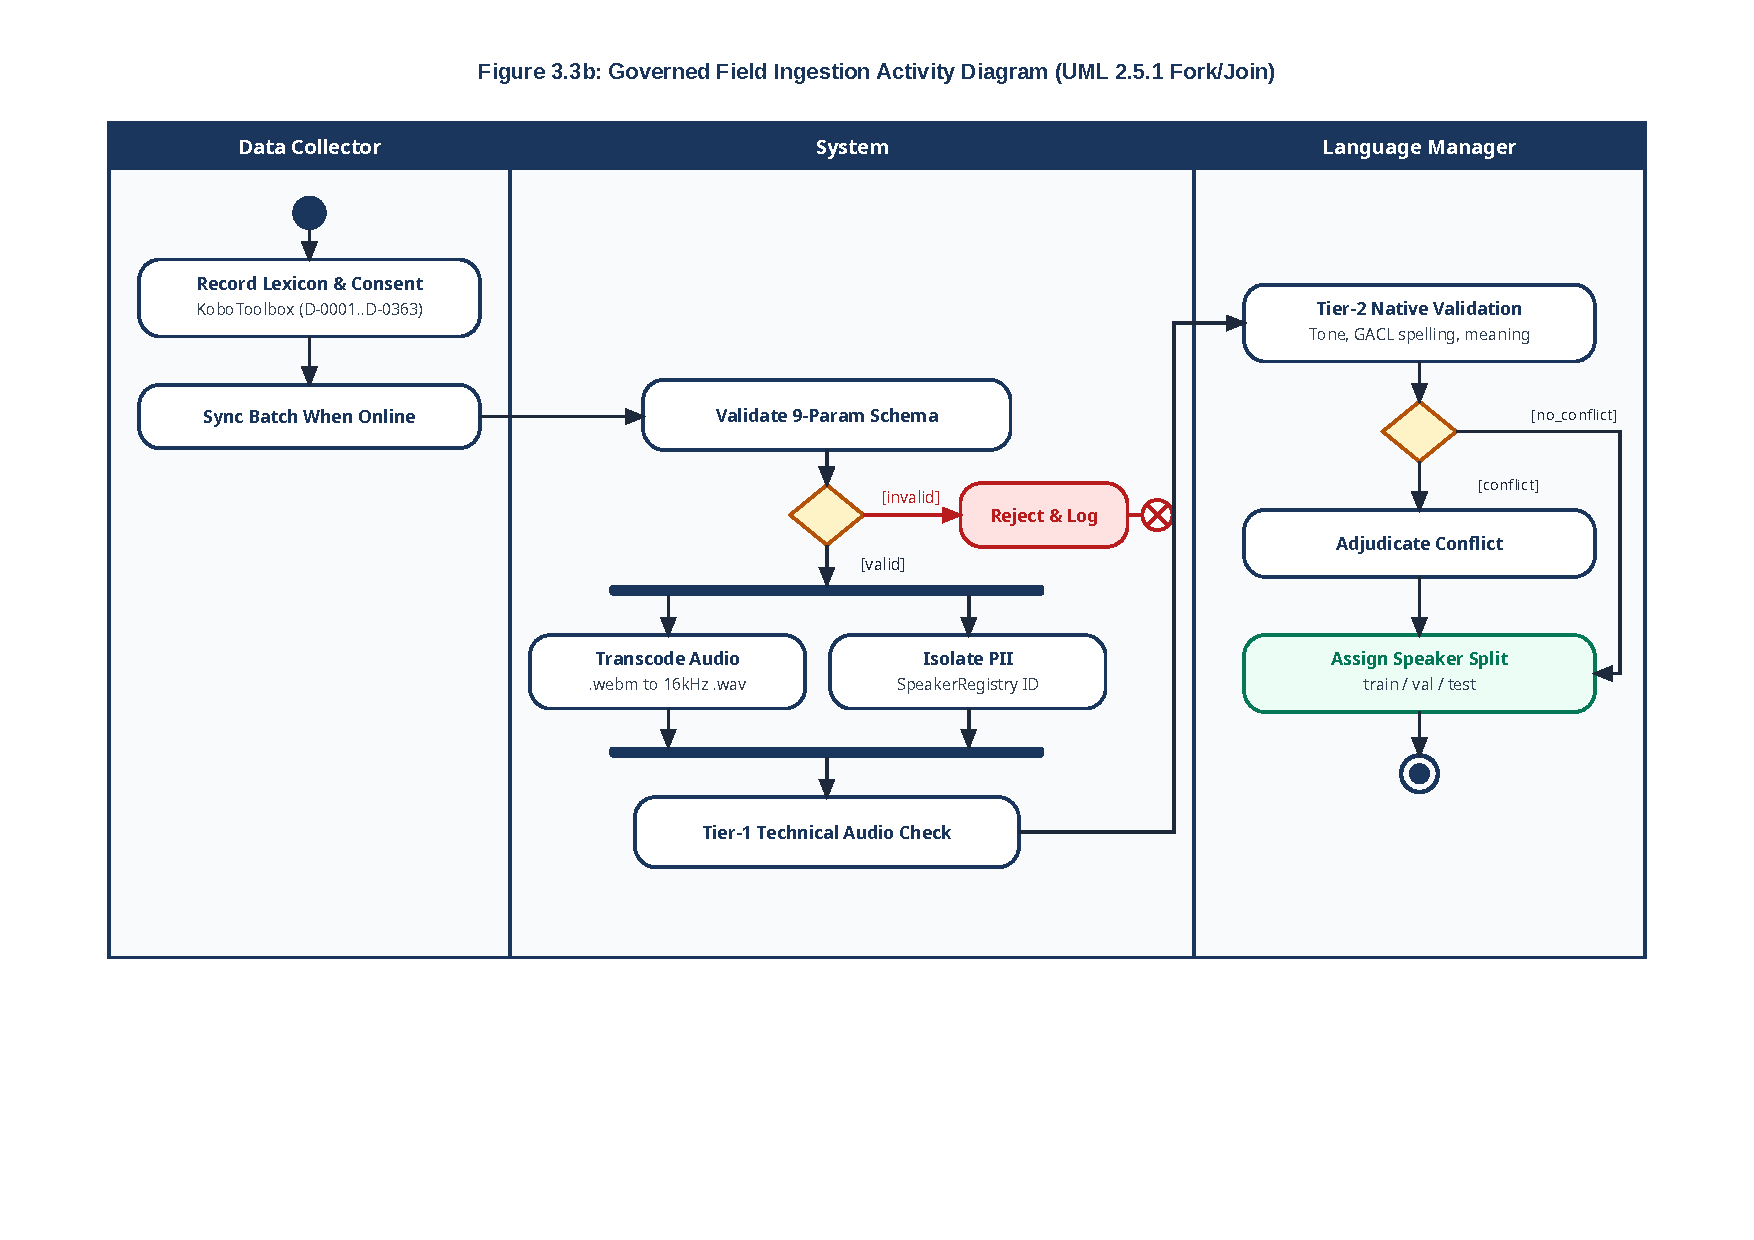
\includegraphics[width=0.48\textwidth]{assets/img/Figure_3_3b_Ingestion_Activity.pdf}
\caption{Figure 3.3: KCS Media Studio Dynamic Behavioral Models: (Left) Figure 3.3a Captioning and Alignment Sequence Diagram with alt-branch for zero-fabrication graceful degradation; (Right) Figure 3.3b Governed Field Ingestion Activity Diagram with Fork/Join synchronization and relational speaker split assignment.}
\label{fig:report_dynamic_models}
\end{figure*}

\subsubsection{UML Dynamic Behavioral Models (Figure~\ref{fig:report_dynamic_models})}
\label{sec:report_uml:dynamic}
System behavior and data flow are captured through two complementary dynamic models: a Sequence Diagram modeling the real-time caption editing flow, and an Activity Diagram modeling the governed ingestion of field recordings.

\paragraph{1. Captioning and Alignment Sequence Diagram (Figure~\ref{fig:report_dynamic_models} Left / Figure~3.3a):}
This sequence traces the asynchronous message exchange among four lifeline participants: the \texttt{User/Client}, the \texttt{:BrowserWorkspace (React)}, the \texttt{:FastAPIController}, and the \texttt{:ASRInferenceService (Whisper/CTC)}:
\begin{enumerate}
    \item \textbf{Media Upload:} The user selects a source video and specifies the target language and dialect (\texttt{uploadVideo(file, lang, dialect)}).
    \item \textbf{Instant Client-Side Waveform Rendering:} The browser workspace intercepts the media and invokes the browser-native \textbf{Web Audio API}~\cite{w3c2021webaudio} via \texttt{decodeWebAudio()} and \texttt{renderCanvas()}. An interactive, scrubbable sound waveform is rendered on an HTML5 Canvas in under 15 milliseconds, giving the user immediate visual feedback without waiting for server uploads.
    \item \textbf{Asynchronous Transcription Request:} The client dispatches \texttt{requestDraftCaptions(asset\_id, lang)} to the FastAPI controller, which delegates the job to the containerized ASR microservice via \texttt{transcribeAndAlign(wav\_uri, lang)}.
    \item \textbf{Graceful Degradation via Alternative Frame (alt):}
    \begin{itemize}
        \item \textbf{Success Branch [inference\_ok == true]:} The ASR service returns aligned segments (\texttt{rawSegments(text, start\_ms, end\_ms)}). The controller applies NFC composition, attaches dialect glossary hints, and returns \texttt{draftSegments(nfc\_text, length\_warning)}. The editor can then interactively refine tone markings, verify timing boundaries, and export WebVTT subtitles.
        \item \textbf{Failure Branch [else: timeout OR unsupported\_lang]:} If the GPU microservice is overloaded, unreachable, or times out, the service returns an explicit error status (\texttt{errorStatus(NO\_FABRICATED\_TEXT)}). The controller relays an \texttt{explicitFailureNotice()} to the browser. Crucially, the platform \textbf{never fabricates placeholder words or hallucinates output}. Instead, the browser workspace keeps all existing subtitle work safe and automatically activates the manual waveform timing mode, allowing the editor to place cue boundaries by eye using visual speech energy peaks on the canvas.
    \end{itemize}
\end{enumerate}

\paragraph{2. Governed Field Ingestion Activity Diagram (Figure~\ref{fig:report_dynamic_models} Right / Figure~3.3b):}
This activity diagram tracks the workflow of field recordings across three organizational swimlanes (\textit{Data Collector}, \textit{System}, and \textit{Language Manager}):
\begin{enumerate}
    \item \textbf{Offline Collection:} The Data Collector records native speakers in remote villages using KoboToolbox, capturing audio responses and verbal consent across our 363 standardized prompts.
    \item \textbf{Batch Synchronization:} When mobile connectivity becomes available, recordings are transmitted in batches to the backend.
    \item \textbf{Schema Validation and Transcoding:} The system automatically validates each incoming file against our 9-parameter naming convention. Non-conforming files branch to \texttt{[invalid] Reject \& Log} for audit review. Conforming files branch to \texttt{[valid] Transcode Audio (.webm to 16\,kHz .wav)} and \texttt{Isolate PII (SpeakerRegistry ID)}, stripping speaker names and phone numbers to guarantee privacy.
    \item \textbf{Concurrent Validation (UML Fork Node):} Execution reaches a UML Fork Node, splitting into two parallel review streams:
    \begin{itemize}
        \item \textit{Tier-1 Technical Check:} Automated evaluation of signal clarity, clipping, and Signal-to-Noise Ratio (SNR).
        \item \textit{Tier-2 Native Linguistic Check:} Qualitative evaluation by a Language Manager, verifying that vowel tones, consonants, and dialect vocabulary match community linguistic standards.
    \end{itemize}
    \item \textbf{Synchronization and Conflict Resolution (UML Join Node):} A UML Join Node gathers both reviews. If validators disagree, the workflow routes to \texttt{[conflict] Adjudicate Conflict} for expert review. If both reviews pass, the recording branches to \texttt{[no\_conflict] Assign Speaker Split}. Here, recordings are partitioned into training, validation, or test sets strictly at the speaker level, ensuring that no speaker appears in both training and test sets.
\end{enumerate}

\begin{figure*}[!t]
\centering
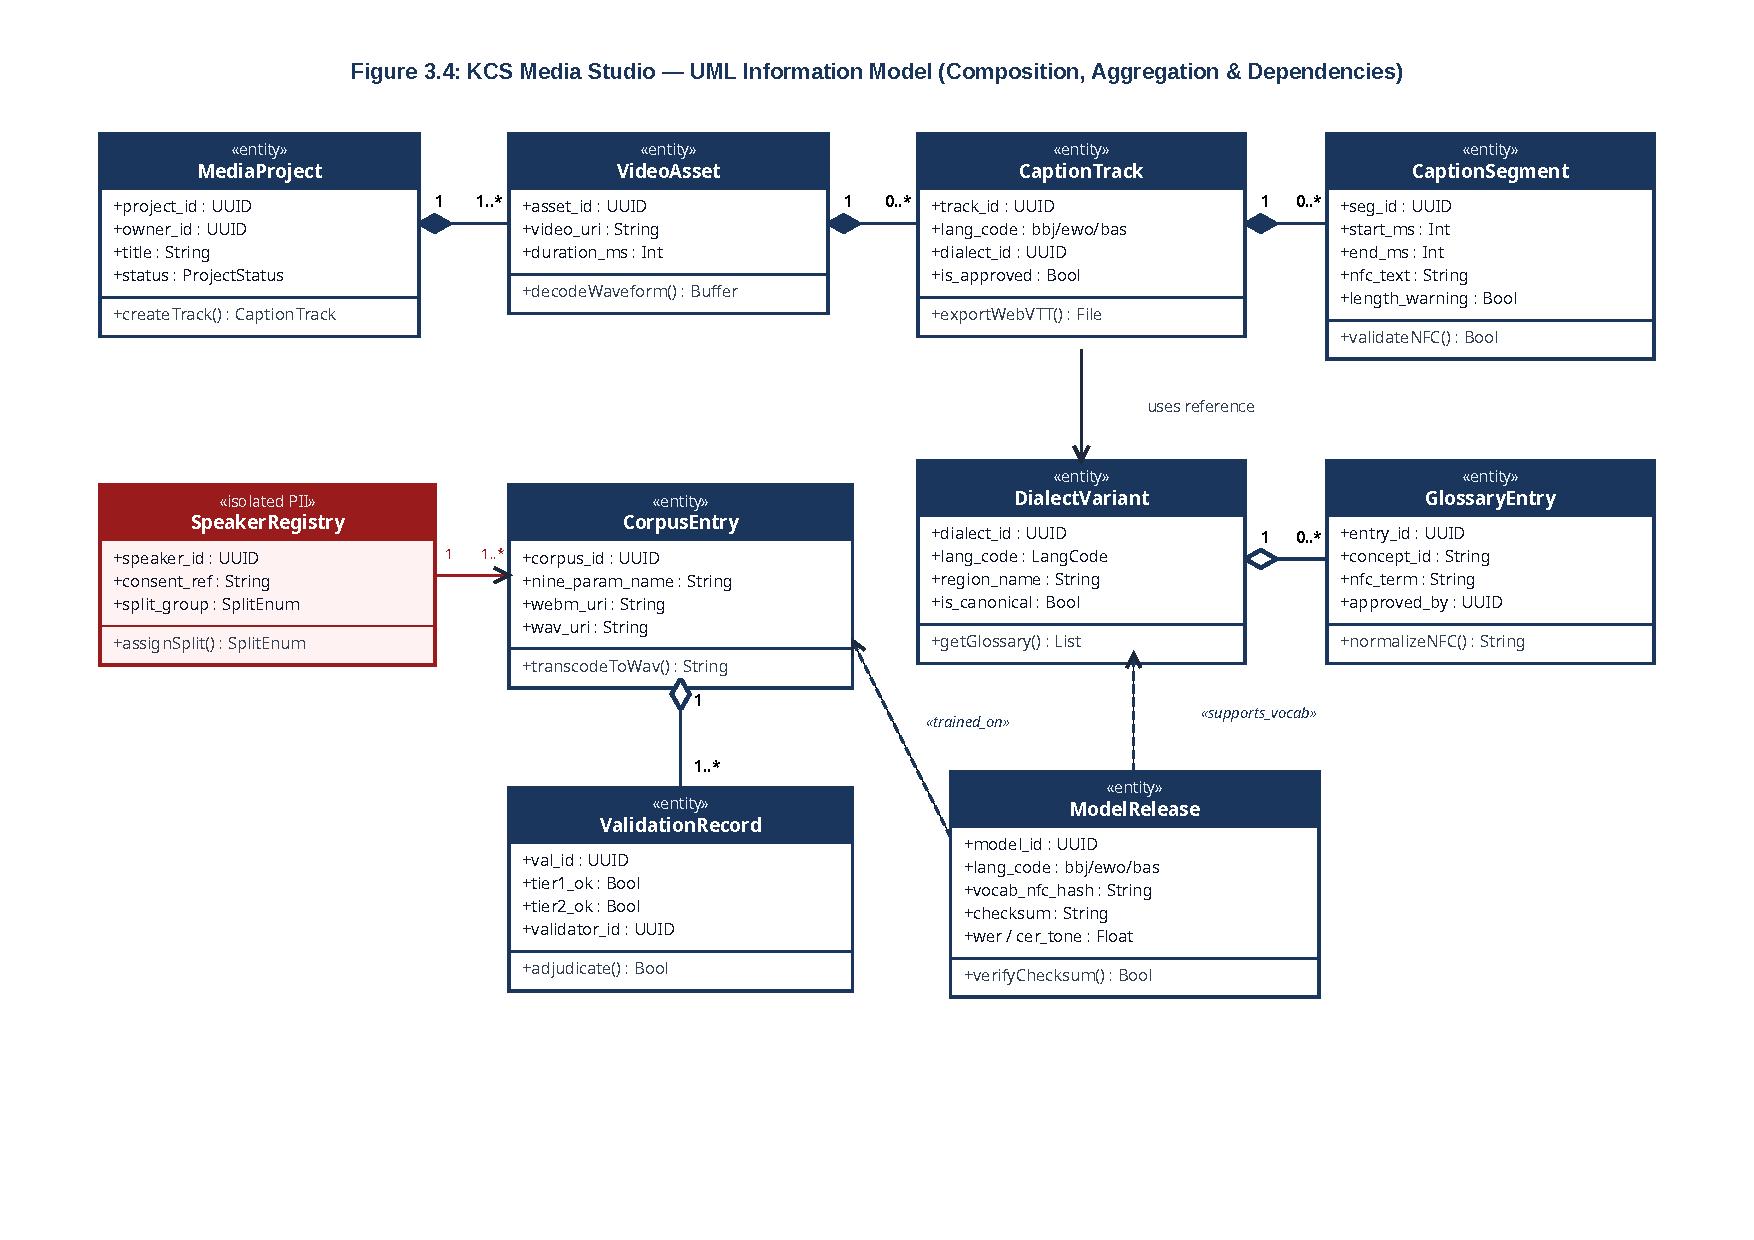
\includegraphics[width=0.84\textwidth]{assets/img/Figure_3_4_Information_Model.pdf}
\caption{Figure 3.4: KCS Media Studio — UML Information Model, illustrating entity classes, attributes, methods, multiplicities, composition hierarchies, isolated PII entities, and model release relationships.}
\label{fig:report_information_model}
\end{figure*}

\subsubsection{UML Domain Information Model (Figure~\ref{fig:report_information_model})}
\label{sec:report_uml:information}
The Information Model defines the core business entities, their internal attributes and methods, their structural relationships, and the multiplicity constraints governing the platform:
\begin{itemize}
    \item \textbf{\texttt{MediaProject} (Root Aggregate):} Represents a complete subtitling project. Contains attributes \texttt{project\_id: UUID}, \texttt{owner\_id: UUID}, \texttt{title: String}, and \texttt{status: ProjectStatus}. It maintains a $1$-to-$1..*$ composition hierarchy with \texttt{VideoAsset} and a $1$-to-$0..*$ composition with \texttt{CaptionTrack}. Deleting a project automatically cascades to its associated assets and subtitle cues.
    \item \textbf{\texttt{VideoAsset}:} Represents the ingested source media. Stores \texttt{asset\_id: UUID}, \texttt{video\_uri: String}, and \texttt{duration\_ms: Int}, providing the client-side method \texttt{decodeWaveform(): Buffer} for real-time waveform visualization.
    \item \textbf{\texttt{CaptionTrack}:} Manages a complete set of timed subtitles for a specific language (\texttt{lang\_code: bbj / ewo / bas}) and regional dialect (\texttt{dialect\_id: UUID}). It tracks approval state (\texttt{is\_approved: Bool}) and exposes the \texttt{exportWebVTT(): File} method. A project can hold multiple tracks simultaneously, enabling seamless multi-language captioning for the same video.
    \item \textbf{\texttt{CaptionSegment}:} An individual timed subtitle cue. Attributes include \texttt{seg\_id: UUID}, \texttt{start\_ms: Int}, \texttt{end\_ms: Int}, \texttt{nfc\_text: String}, and \texttt{length\_warning: Bool}. The method \texttt{validateNFC(): Bool} validates that all characters adhere to Unicode NFC canonical composition prior to persistence.
    \item \textbf{\texttt{DialectVariant} and \texttt{GlossaryEntry}:} Handles regional dialect diversity. \texttt{DialectVariant} represents regional dialects (e.g., Yaound\'e vs. rural Ewondo), holding a $1$-to-$0..*$ composition of \texttt{GlossaryEntry} records. Each glossary entry maps an abstract concept ID to an approved, localized tone-marked spelling, giving translators immediate vocabulary suggestions.
    \item \textbf{\texttt{SpeakerRegistry} (Isolated PII):} To uphold CARE data governance~\cite{carroll2020care}, speaker personal data is strictly separated from acoustic data. Attributes include \texttt{speaker\_id: UUID}, encrypted \texttt{consent\_ref}, and \texttt{split\_group: SplitEnum}. It maintains a $1$-to-$1..*$ relationship with \texttt{CorpusEntry}, enforcing speaker-level dataset isolation.
    \item \textbf{\texttt{CorpusEntry} and \texttt{ValidationRecord}:} Represents verified field recordings. \texttt{CorpusEntry} stores the 9-parameter filename, raw audio URI, and transcoded 16\,kHz WAV URI. Each entry is linked to a \texttt{ValidationRecord} storing Tier-1 technical metrics, Tier-2 linguistic reviews, and adjudication logs.
    \item \textbf{\texttt{ModelRelease}:} Represents a versioned ASR model checkpoint. Stores \texttt{model\_id: UUID}, \texttt{lang\_code}, \texttt{vocab\_nfc\_hash}, \texttt{checksum}, \texttt{wer}, and \texttt{cer\_tone}. It maintains traceability links to the exact training corpus (\texttt{«trained\_on»}) and supported vocabulary (\texttt{«supports\_vocab»}).
\end{itemize}

\begin{figure*}[!t]
\centering
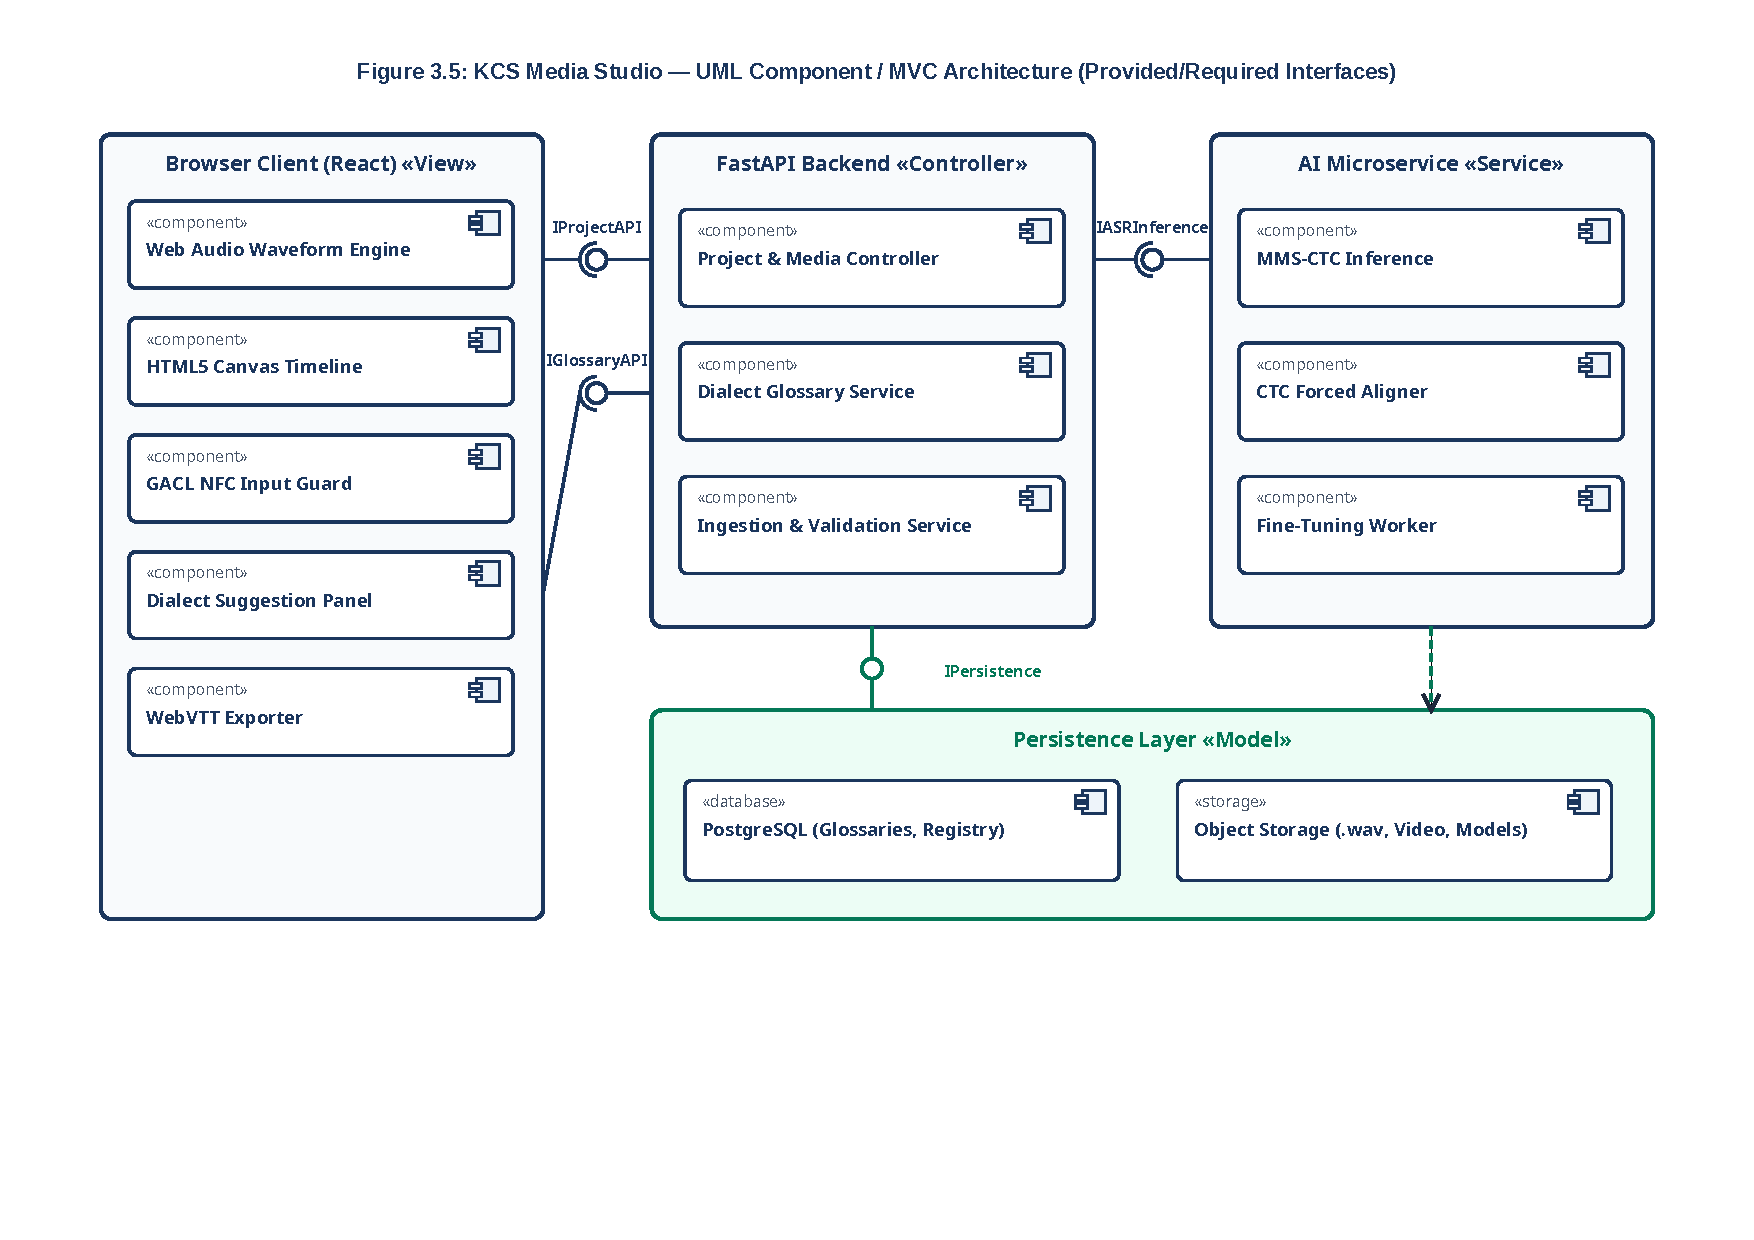
\includegraphics[width=0.84\textwidth]{assets/img/Figure_3_5_Component_MVC.pdf}
\caption{Figure 3.5: KCS Media Studio — UML Component / MVC Architecture Diagram, illustrating Provided and Required Interface contracts (IProjectAPI, IGlossaryAPI, IASRInference, IPersistence) across View, Controller, Service, and Persistence layers.}
\label{fig:report_component_mvc}
\end{figure*}

\subsubsection{UML Component and Layered MVC Model (Figure~\ref{fig:report_component_mvc})}
\label{sec:report_uml:component}
The Component Diagram details the software architecture organized into clean, decoupled layers following the Model-View-Controller (MVC) pattern. Clear interface contracts govern communication across layers:
\begin{itemize}
    \item \textbf{View Layer (Client Browser SPA — React):} Executes entirely within modern web browsers on commodity hardware. It contains five modular components: the \textit{Web Audio Waveform Engine} (real-time decoding), the \textit{HTML5 Canvas Timeline} (visual timeline navigation), the \textit{GACL NFC Input Guard} (virtual tone keyboard and Unicode normalization), the \textit{Dialect Suggestion Panel} (regional vocabulary hints), and the \textit{WebVTT Exporter} (subtitle file compilation). The View communicates with the backend exclusively through the required interface \texttt{IProjectAPI}.
    \item \textbf{Controller Layer (Application Server — FastAPI):} Implements interface \texttt{IProjectAPI}. It contains the \textit{Project \& Media Controller} (session handling and request routing), the \textit{Dialect Glossary Service} (dictionary lookup and dialect matching), and the \textit{Ingestion \& Validation Service} (field submission processing). The Controller delegates speech recognition tasks via the required interface \texttt{IASRInference}, queries dictionaries via \texttt{IGlossaryAPI}, and manages database state via \texttt{IPersistence}.
    \item \textbf{Service Layer (ASR Inference Microservice — PyTorch):} Provides interface \texttt{IASRInference}. It encapsulates the fine-tuned \textit{Whisper ASR Inference Engine}, the \textit{CTC Forced Aligner} (mapping phonetic tokens to exact millisecond audio frames), and an asynchronous \textit{Fine-Tuning Worker}. Isolating compute-intensive AI operations into an independent microservice ensures that transcription workloads never degrade web UI responsiveness.
    \item \textbf{Persistence Layer (Model):} Provides interface \texttt{IPersistence}. It manages structured data in the \textit{PostgreSQL Relational Database} (projects, users, captions, glossaries, validation audits) and large binary files in \textit{Object Storage} (raw video, extracted audio, and model checkpoints).
\end{itemize}

\begin{figure*}[!t]
\centering
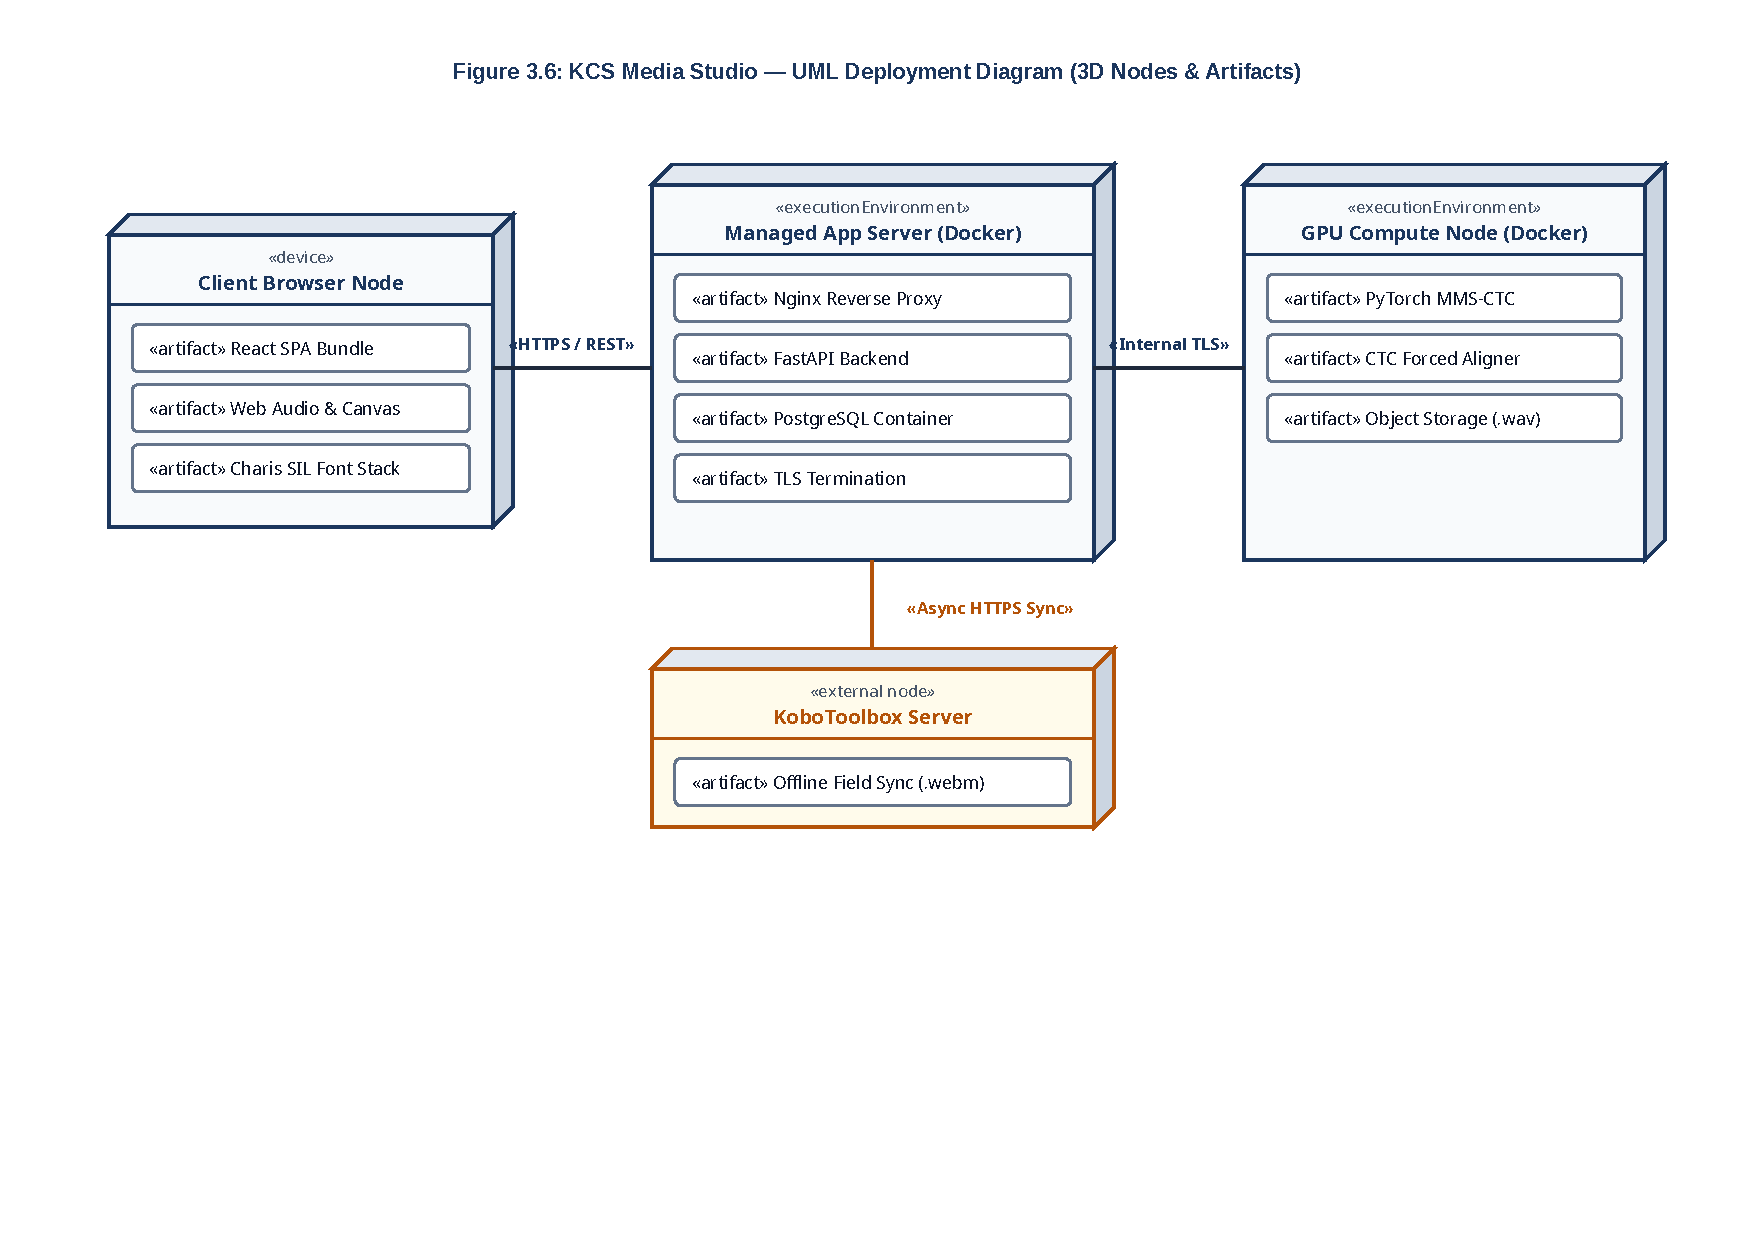
\includegraphics[width=0.84\textwidth]{assets/img/Figure_3_6_Deployment_Diagram.pdf}
\caption{Figure 3.6: KCS Media Studio — UML Deployment Diagram, depicting 3D execution nodes, containerized Docker artifacts, GPU compute infrastructure, and secure network communication protocols.}
\label{fig:report_deployment_diagram}
\end{figure*}

\subsubsection{UML Deployment Model (Figure~\ref{fig:report_deployment_diagram})}
\label{sec:report_uml:deployment}
The Deployment Diagram defines the physical and virtual runtime topology, illustrating execution environment nodes, containerized artifacts, and communication links:
\begin{itemize}
    \item \textbf{Client Browser Node («device»):} Commodity client machines (laptops, desktops) running modern web browsers. It hosts the compiled \textit{React SPA Bundle}, the \textit{Web Audio and Canvas Engine}, and the embedded \textit{Charis SIL Font Stack}, ensuring consistent rendering of all GACL phonetic characters across operating systems without requiring users to install external fonts manually.
    \item \textbf{Managed App Server Node («executionEnvironment», Docker):} Cloud or institutional server running three Docker containers:
    \begin{itemize}
        \item \textit{Nginx Reverse Proxy Container:} Terminates external client connections with TLS 1.3 encryption, serving static frontend assets and routing API requests.
        \item \textit{FastAPI Application Container:} Executes our Python backend controllers, business logic, and security middleware.
        \item \textit{PostgreSQL Database Container:} Encrypted relational database storing application metadata and dialect glossaries.
    \end{itemize}
    \item \textbf{GPU Compute Node («executionEnvironment», Docker):} Dedicated server equipped with an NVIDIA GPU for accelerated deep learning inference. It hosts containers for the \textit{PyTorch Whisper / CTC Inference Service}, the \textit{FFmpeg Audio Processor}, and \textit{MinIO Object Storage}. Connected to the application server via a private, firewalled network over internal TLS.
    \item \textbf{KoboToolbox Server Node («external node»):} Secure humanitarian cloud instance receiving mobile survey submissions from Android devices in the field and synchronizing data with the application server via asynchronous HTTPS calls.
\end{itemize}

\subsubsection{UML Models Traceability Matrix}
\label{sec:report_uml:matrix}
As detailed in the comprehensive requirements traceability matrix (Table~\ref{tab:requirements_traceability_report}), each UML architectural diagram, component stereotype, and interface contract maps directly to our verified user needs, functional requirements (FR-01 to FR-10), quality attributes (QR-01 to QR-06), and core research questions.
\subsection{Ethics, Data Governance, Security, Accessibility, and Pre-Implementation Evaluation Plan}
\label{sec:chap3_governance}

\subsubsection{Ethics and Indigenous Linguistic Sovereignty}
\label{sec:chap3_gov_ethics}
Linguistic research involving indigenous minority languages requires adherence to ethical data sovereignty frameworks, specifically the \textbf{CARE Principles for Indigenous Data Governance} (Collective Benefit, Authority to Control, Responsibility, and Ethics)~\cite{carroll2020care}:
\begin{itemize}
    \item \textbf{Informed Consent Protocol:} Field enumerators obtain signed or audio-recorded informed consent in the contributor's native language prior to recording. Contributors are explicitly informed of intended research usage, open model training, and non-commercial licensing.
    \item \textbf{Unconditional Right of Withdrawal:} Contributors retain full autonomy over their voice recordings. Under requirement \textbf{QR-04}, participants may request withdrawal at any time; upon receipt of a withdrawal reference, the system triggers an automated deletion job purging all linked audio assets and re-partitioning dataset manifests.
    \item \textbf{Non-Commercial Cultural Protection:} Linguistic corpora and trained model checkpoints are released under Creative Commons non-commercial attribution licenses (CC BY-NC 4.0), preventing commercial exploitation of community cultural assets without community benefit.
\end{itemize}

\subsubsection{Security Architecture and PII Isolation}
\label{sec:chap3_gov_security}
The security architecture enforces defense-in-depth across storage, computation, and transmission:
\begin{itemize}
    \item \textbf{Speaker Registry Pseudonymization:} Biometric voice samples are strictly separated from participant identities. Personal identifying information (names, phone numbers, GPS coordinates) is encrypted and restricted to the \texttt{SpeakerRegistry} table, while acoustic audio files are referenced solely by anonymous cryptographic hashes and demographic tokens (fulfilling \textbf{FR-07}).
    \item \textbf{Authentication and Role-Based Access Control (RBAC):} The FastAPI backend enforces OAuth2 with JSON Web Tokens (JWT) encrypted via HS256. User permissions are partitioned across four granular roles: \textit{Caption Editor} (read/write access to assigned media projects), \textit{Language Manager} (read/write access to glossaries, adjudication controls, and validation queues), \textit{Data Collector} (write-only ingestion permissions), and \textit{Platform Administrator} (infrastructure and model release deployment controls).
    \item \textbf{Cryptographic Transit and Rest Encryption:} All external traffic is terminated via TLS 1.3 using modern cipher suites on the Nginx reverse proxy. Internal traffic between the Managed App Server and GPU Compute Node traverses an isolated virtual network encrypted via internal TLS. Media assets and PostgreSQL volumes are encrypted at rest using AES-256.
\end{itemize}

\subsubsection{Accessibility and Typographic Conformance}
\label{sec:chap3_gov_accessibility}
To ensure the editing workspace is accessible to diverse users, including individuals with visual or motor impairments, the user interface adheres to W3C Web Content Accessibility Guidelines (WCAG 2.1 Level AA)~\cite{norman1986user}:
\begin{itemize}
    \item \textbf{Full Keyboard Operability:} All timeline navigation and editing tasks operate entirely via keyboard shortcuts without requiring mouse interaction: \texttt{Space} (toggle video playback), \texttt{J/K/L} (shuttle backwards, pause, shuttle forward), \texttt{Tab} and \texttt{Shift+Tab} (navigate between subtitle cues), \texttt{Ctrl+Enter} (split segment at playhead), and \texttt{Ctrl+S} (save project).
    \item \textbf{Typographic Safety and Contrast:} Visual styling enforces a minimum text-to-background contrast ratio of $7:1$ for subtitle text against video bounding boxes. The Charis SIL web font stack renders stacked diacritics with dynamic CSS line-height calculations (minimum 1.6x font size), eliminating glyph collisions and preventing font clipping.
    \item \textbf{Screen Reader Compatibility:} Interactive elements feature explicit WAI-ARIA labels (e.g., \texttt{aria-label="Audio Waveform Timeline"}), providing descriptive status announcements during ASR transcription, dialect switching, and WebVTT export operations.
\end{itemize}

\subsubsection{Pre-Implementation Evaluation Plan}
\label{sec:chap3_gov_evalplan}
To validate the system architecture empirically prior to production deployment, we formalize three testable research hypotheses to be evaluated in Chapter~5:
\begin{itemize}
    \item \textbf{Hypothesis $H_1$ (ASR Error Reduction via Character-Level CTC):} Evaluating fine-tuned MMS-CTC on our double-validated conversational Cameroonian test corpus will achieve a Word Error Rate below $35\%$ and a tonemic Character Error Rate below $15\%$, representing a $>50\%$ relative error reduction over unadapted baselines ($74.2\%\text{--}86.5\%$ WER).
    \item \textbf{Hypothesis $H_2$ (Subtitling Throughput Acceleration):} Utilizing KCS Media Studio with automated ASR drafting, waveform boundary snapping, and dialect glossaries will reduce total subtitling effort from the unassisted baseline of 10.8 minutes down to \textbf{under 3.5 minutes of labor per minute of finished video} (a $>65\%$ throughput efficiency improvement).
    \item \textbf{Hypothesis $H_3$ (Cognitive Workload and Usability Approval):} In standardized user testing with 15 native translators, the system will achieve an empirical System Usability Scale (SUS) score exceeding \textbf{80/100} and reduce NASA-TLX cognitive frustration scores by $>40\%$ compared to conventional manual subtitling workflows.
\end{itemize}

\paragraph{Controlled Evaluation Protocol for Chapter 5.}
The experimental protocol recruits 15 fluent native speakers (5 for Ewondo, 5 for Gh\textopeno m\'al\'a', 5 for Basaa) spanning professional translators, educators, and community creators. Participants complete counterbalanced subtitling trials: Task A uses standard commercial software (Premiere Pro / Subtitle Edit), while Task B uses KCS Media Studio on standardized 5-minute educational video clips. Total task completion time, character correction edit counts, NASA-TLX subjective cognitive workload ratings, and SUS survey scores are logged and analyzed using paired two-tailed $t$-tests and ANOVA ($\alpha = 0.05$).

\subsection{Chapter Summary}
\label{sec:chap3_summary}
This chapter executed the Theory Building phase of the Nunamaker SDIS framework by establishing the comprehensive system architecture and formal models for the Kingdom Communication Solutions (KCS) Media Studio. Grounded in four empirical UCD evidence records and ten practical challenges, we derived ten functional requirements (FR-01 to FR-10) and six quality requirements (QR-01 to QR-06). We specified the system boundary and layered MVC architecture, presented the smallest coherent set of six complementary UML diagrams (context, use case, sequence, activity, information model, component MVC, and deployment), defined data governance and security frameworks, and formalized our pre-implementation evaluation plan. Chapter~4 will detail the concrete software implementation of these architectural models.

\FloatBarrier
\clearpage

\nocite{*}
\printbibliography[heading=bibintoc]

\end{document}
